\chapter{The Effective Theory} \label{chap4}

Having presented the challenges and difficulties in simulating strongly
interacting fermions, especially in the dense regime, we will introduce an
effective theory that handles some of these problems, while reproducing the full
theory in a certain parameter region. We will see that although simulations of
the effective theory still suffer from the side effects of the sign problem
(e.g. complex actions), the sign problem is in essence weak enough that
reweighting can be readily applied.

The work in this thesis builds on previous work with the effective theory while
pushing the derivation further and introducing analytic tools, which we will
cover in the next chapter.

In the present chapter we will first introduce the effective theory before
introducing two expansion schemes that facilitate the computation of the theory.
These are namely the \emph{character expansion}, mentioned in
\secref{sec:group_intro}, and the \emph{hopping parameter expansion} for heavy
fermions. We round off the chapter with a discussion on the numerical evaluation
of the effective theory.

\section{The effective theory - \texorpdfstring{\itshape Introduction}{Introduction}}

The essence of the derivation of the effective theory is to integrate out some
of the degrees of freedom analytically. This will both ease the burden of the
numerical evaluation, having fewer degrees of freedom left to vary, which in
turn lessens the sign problem. The sign problem will be milder due to the fact that
many, or as we will see, most, of the fluctuations cancel exactly, as they
should. In this we will integrate the spatial gauge links of the partition
function
%
\begin{equation}
  \mathcal{Z} = \int \prod_{x, \mu} \mathrm{d} U_{\mu}(x) \, \det Q \, [U_{\mu}] \,
    e^{-\mathcal{S}_g[U_{\mu}]}
    \equiv \int \prod_{x} \mathrm{d} U_0(x) \,
    e^{-\mathcal{S}_{\text{eff}}[U_0]},
\end{equation}
%
which defines the effective action to be
%
\begin{equation} \label{eq:eff_action_def}
  \mathcal{S}_{\text{eff}} = - \log \int \prod_{x, i} \mathrm{d} U_i(x) \, \det
    Q \, [U_{\mu}] \, e^{-\mathcal{S}_g [U_{\mu}]}.
\end{equation}
%
The integrals over the spatial gauge links $U_i(x)$ is unfortunately not
something we can evaluate analytically without the aid of approximations. We
will therefore introduce two expansion schemes and work towards deriving the
effective theory such that it reproduces the exact expansion coefficients of the
full lattice gauge theory in the end.

\section{The character expansion} \label{sec:char_exp}

The first expansion we will apply is the character expansion introduced in 
\secref{sec:group_intro}. In the form of an exact equality, it is not of much
help. Nevertheless, from the character expansion of the single plaquette gauge
contribution
\footnote{We will from this point onward assume that the gauge group is SU$(N_c)$
  and that the fermions transform under the fundamental representation, unless
  stated otherwise.}
%
\begin{equation}
  e^{-\beta (1 - \frac{1}{N_c} \text{Re} \tr U_p)} = u_0(\beta) \bigg(1 +
  \sum_{r \neq 0} d_r\, u_r(\beta)\, \chi_r(U_p) \bigg),
\end{equation}
%
we see that the character expansion coefficients are dependent on the lattice
gauge coupling $\beta$. It can be easily seen that the higher dimensional
representations come with a higher power of this coupling. A natural ordering
therefore arises if one expands around the infinite coupling limit,
$g\to\infty$, $\beta\to0$. This expansion scheme is aptly named the \emph{strong
  coupling expansion}, and has been the focus of numerous studies for the past
decades, also having been picked up in recent years by groups studying conformal
field theories. Introductions to the field can be found in \cite{Drouffe:1983fv}
and \cite{montvay1997quantum}.

The lowest order character expansion coefficient, namely that of the fundamental
representation, has for SU$(3)$ been calculated to high orders
%
\begin{align}
  u_F(\beta) &= \frac{1}{N_c} \frac{\int \mathrm{d} g\, \tr g\, e^{-\frac{\beta}{2 N_c}
    ( \tr g + \tr g^{\dagger})}}{\int \mathrm{d} g\: e^{-\frac{\beta}{2 N_c}
    ( \tr g + \tr g^{\dagger})}} \nonumber\\
  &\hskip1em= \frac{
    x + \frac{1}{2} x^2 + x^3 + \frac{5}{8} x^4 + \frac{13}{24} x^5 + \mathcal{O}(x^6)%
  }{%
    1 + x^2 + \frac{1}{3} x^3 + \frac{1}{2} x^4 + \frac{1}{4} x^5 + \mathcal{O}(x^6)%
  }, \hskip2ex x=\frac{\beta}{2 N_c}.
\end{align}
%
To leading order $u_F(\beta) \approx \frac{\beta}{2 N_c^2}$, and we
therefore use $u_F$ as our expansion parameter rather than $\beta$.
The characters are in fact always smaller than or equal to $1$, and therefore
does an excellent job as an expansion parameter.  The character expansion only
permits a single plaquette from any representation to be placed at each
position, making order counting easier than a standard Taylor expansion of the
gauge action.

\section{Pure gauge effective theory} \label{sec:pure-gauge-theory}

With the character expansion at hand we can evaluate the pure gauge
contributions to the effective action. Ignoring the quark contribution, the
effective action is
%
\begin{equation}
  e^{-\mathcal{S}_{\text{eff}}} = \int \big[ \mathrm{d} U \big]_i \, \prod_p
    \bigg(1 + \sum_{r \neq 0} d_r u_r(\beta) \chi_r (U_p) \bigg),
\end{equation}
%
where we have introduced the shorthand integration measure $\big[ \mathrm{d} U
\big]_i = \prod_{x,i} \mathrm{d} U_{i}(x)$.  Expanding the product over the
plaquettes gives a sum of terms which are of the form
%
\begin{equation}
  d_{r_1} u_{r_1}(\beta) \chi_{r_1}(U_{p_1}) \, 
  d_{r_2} u_{r_2}(\beta) \chi_{r_2}(U_{p_2}) \, \cdots
\end{equation}
%
where if one or more of the plaquettes in a term has a link that fall on
$(x,\mu)$, gives the integral
%
\begin{equation}
  \int \mathrm{d} U_{\mu}(x) \, \chi_{r_1} \big(U_{s_1} U_{\mu}(x) \big) \,
    \chi_{r_2} \big(U_{s_2} U_{\mu}(x) \big) \, \cdots,
\end{equation}
%
where $U_{s_i}$ is the remaining \emph{staple} after the link $U_{\mu}(x)$ has
been factored out of the plaquette. One approach to solving these integrals is
to carry out the Kronecker product of the representation matrices and
decompose them to their irreducible representations using the Clebsch-Gordan
coefficients. We see that only products of characters whose Clebsch-Gordan
series contains the trivial representation do not vanish due to the identity
%
\begin{equation}
  \int \mathrm{d} g \, \chi_r (g) = \delta_{r,0}.
\end{equation}
%
On top of restricting the valid plaquette combinations sharing a link, it also
restricts the graphs created from plaquette combinations to ones that have no
boundaries. On an infinite lattice the lowest order contribution would therefore
come from combining six fundamental plaquettes into a cube.

For finite lattices, the periodic boundary can be utilised to create closed
surfaces. In fact, only graphs periodic in the temporal direction
contribute to the finite temperature observables as the non-periodic ones can be
normalised out. Since we only integrate spatial links, the contributing graphs
need only have closed surfaces in the spatial directions. The lowest order
contribution to the effective action comes from a strip of plaquettes spanning
the temporal direction as shown in \figref{fig:plaquette-strip}. Since only two
links meet at all the spatial sites we need only the integral
%
\begin{equation}
  \int \mathrm{d} U \: \chi_r(V U) \: \chi_s(W U^{-1})
    = \delta_{r,s} \frac{1}{d_r} \chi_r (V W),
\end{equation}
%
which can be represented graphically as
%
\begin{equation} \label{eq:gauge-link-integral-graphic}
  \int \mathrm{d} U \;%
  \begin{tikzpicture}[baseline={(base)}]
    \coordinate (base) at (0,.35);
    \draw[link line] (0,0) rectangle (2,1);
    \draw[link] (0,0) -- (0,1)
      node[midway,left=1mm,inner sep=0pt,ColourBase,scale=0.8] {$V$};
    \draw[link] (2,1) -- (2,0)
      node[midway,right=1mm,inner sep=0pt,ColourBase,scale=0.8] {$W$};
    \draw[link double] (1,0) -- (1,1)
      node[midway,right=1mm,inner sep=0pt,ColourBase,scale=0.8] {$U$};
  \end{tikzpicture}
  \,=\, \frac{1}{d_r} \;
  \begin{tikzpicture}[baseline={(base)}]
    \coordinate (base) at (0,.35);
    \draw[link line] (0,0) rectangle (2,1);
    \draw[link] (0,0) -- (0,1)
      node[midway,left=1mm,inner sep=0pt,ColourBase,scale=0.8] {$V$};
    \draw[link] (2,1) -- (2,0)
      node[midway,right=1mm,inner sep=0pt,ColourBase,scale=0.8] {$W$};
  \end{tikzpicture} \,.
\end{equation}

\begin{figure}
  {\centering
    \includegraphics[width=.75\textwidth]{pure_gauge_strip}\par}
  \caption{Lowest order pure gauge contribution to the effective action}
  \label{fig:plaquette-strip}
\end{figure}

Integrating out the spatial links of the strip of plaquettes leaves two
disconnected loops at the neighbouring spatial lattice sites
%
\begin{equation}
  e^{-\mathcal{S}_{\text{eff}}} = 1 + \sum_{\langle \vec{x}, \vec{y} \rangle} u_F^{N_t}
  \big( L_{\vec{x}} L^*_{\vec{y}} + L^*_{\vec{x}} L_{\vec{y}} \big) + \mathcal{O}(u_F^{N_t+4})
\end{equation}
%
where $L$ is the so-called \emph{Polyakov loop}
%
\begin{equation}
  L_{\vec{x}} = \tr \prod_{\mathclap{t=0}}^{\mathclap{N_t-1}} U_0(\vec{x},t) .
\end{equation}
%
We see that the explicit time dependence of the links has disappeared, as the
only degrees of freedom left are full windings. The integral over the effective
action thus simplifies to
%
\begin{equation}
  \mathcal{Z}_{\text{eff}} = \int \big[\mathrm{d} U\big]_0 \,
    e^{-\mathcal{S}_{\text{eff}}[L]} 
  = \int \prod_{\vec{x}} \mathrm{d} L_{\vec{x}} \, \sqrt{\det U_0} \,
    e^{-\mathcal{S}_{\text{eff}}[L]} ,
\end{equation}
%
where $\sqrt{\det U_0}$ is the reduced Haar measure of the group, the calculation of
which is covered in \apxref{sec:haar_measure}. As one can see, the effective
theory is a three dimensional theory of Polyakov loop interactions. To first
order we have a nearest neightbour spin system with an effective coupling
$u_F^{N_t}$.

At higher orders in $\beta$, new effects are introducted through interactions
between loops at higher order representations, next to nearest neighbour
interactions as well as corrections to the nearerst neighbour coupling between
fundamental Polyakov loops. The effects of higher order representations in
Polyakov loop effective theories were studied in \citep{Wozar:2007tz}. The
corrections to the fundamental nearest neighbour coupling was calculated to 
$\mathcal{O}(u_F^{N_t + 10})$ in \citep{Langelage:2010yr} while the effects of
long range interactions was examined in \citep{Bergner:2015rza}.

We will leave the topic of pure gauge effective theories for now as the work in
this thesis is mostly concerned with the cold and dense regime. At low
temperatures the pure gauge contribution is exponentially suppressed as
$\lambda_i \sim u^{n N_t}$, with $n \leq 1$. The pure gauge sector plays no role
in the cold regime, and will be subsequently neglected.

\section{The hopping parameter expansion}

Even for lattice simulations at zero chemical potential, evaluating the fermion
determinant is by far the most expensive operation. For heavy quarks it takes a
close to block diagonal form, while for light quarks the dynamics delocalise,
and no such simplifications appear. It is therefore clear that the analysis of
heavy quarks is of reduced complexity, and an expansion around this limit can be
used to derive an effective theory for heavy quarks. By rescaling the fields, we
see that the quark matrix can be refactored to be
%
\begin{equation}
  Q_{yx} = \delta_{yx} - \kappa H_{yx}, \hskip1em \kappa = \frac{1}{2(4 + am)}
\end{equation}
%
where we have introduced the \emph{hopping parameter} $\kappa$ and the
\emph{hopping matrix} $H$. The hopping matrix for Wilson fermions is
%
\begin{equation}
  H_{yx} = (1 \pm \gamma^0) e^{\pm a\mu} U_{\pm 0}(x) \delta_{y \mp \hat{0},x}
    + \sum_{\mu = \pm 1}^{\pm 3} (1 + \gamma^{\mu}) U_{\mu}(x) \delta_{y-\hat{\mu},x},
\end{equation}
%
where we have chosen $r=1$. We then expand the fermion propagator in powers of
$\kappa$ resulting in
%
\begin{equation}
  Q^{-1}_{yx} = \sum_{n=0}^{\infty} \kappa^n (H^n)_{yx} .
\end{equation}
%
Since every factor of $H$ comes with a $\delta_{y+\hat{\mu},x}$, they symbolise
a single discrete hop on the lattice. The full fermion propagator is
therefore the sum of all fermion lines starting at $x$ and ending at $y$. Due to
the accompanying spin factor, and the fact that $(1 - \gamma^{\mu}) (1 +
\gamma^{\mu}) = 0$, it is restricted to lines with no backtracking.  If the
series is truncated, it is approximated by lines with a specific upper bound for
their length. The fermion matrix can likewise be rewritten using the trace-log
identity
%
\begin{equation}
  \det Q = \exp \big(\tr \log (1 - \kappa H) \big) = \exp \bigg( -\sum_{n=1}^{\infty} \frac{1}{n}
  \kappa^n \tr H^n \bigg).
\end{equation}
%
The trace over $H^n$ gives all closed fermion loops of length $n$ with no
backtracking. In lieu of the hopping expansion we see that the fermion
propagator is the sum of all fermion lines while the determinant is the
exponential of all fermion loops.

\section{Pure fermion effective theory} \label{sec:pure-fermion-eff-theory}

The first step towards deriving an effective three dimensional theory for heavy
quarks and strong coupling is to separate the temporal and spatial hops
%
\begin{equation}
  H_{yx} = T_{yx} + \sum_{i=1}^3 S_{i,yx},
\end{equation}
%
where the temporal and spatial hopping matrices are divided into positive and
negative components: $T = T^+ + T^-$, $S_i = S_i^+ + S_i^-$, and
%
\begin{align}
  T^{\pm}_{yx} &= (1 \pm \gamma^{0}) e^{\pm a\mu} U_{\pm 0}(x)\,
    \delta_{\vec{y},\vec{x}} \, \delta_{t_y, t_x\pm1},\\
  S_{i,yx}^{\pm} &= (1\pm \gamma^i) U_{\pm i}(x) \,
    \delta_{\vec{y},\vec{x}\pm\hat{i}} \,\delta_{t_y,t_x}.
\end{align}
%
The fermion determinant can then be refactored into static and kinematic factors
by factoring out the temporal hopping matrix
%
\begin{equation}
  \det (Q) = \det (1 - \kappa T - \kappa S)
   = \det
  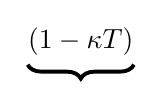
\begin{tikzpicture}[baseline={(trace.base)}]
    \node[inner sep=0pt] (trace) {%
      $(1 - \kappa T)$};
    \draw [
      decorate,
      line width=1.4pt,
      decoration={
        brace,
        mirror,
        amplitude=5pt
      },
      transform canvas={yshift=-.2cm},
    ]
      (trace.south west) -- (trace.south east)
      node[midway,below=5pt] {$\qstat$};
  \end{tikzpicture} \,
    \det
  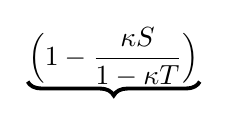
\begin{tikzpicture}[baseline={(trace.base)}]
    \node[inner sep=0pt] (trace) {%
      $\Big(1 - \displaystyle\frac{\kappa S}{1 - \kappa T}\Big)$};
    \draw [
      decorate,
      line width=1.4pt,
      decoration={
        brace,
        mirror,
        amplitude=5pt
      },
      transform canvas={yshift=-.2cm},
    ]
      (trace.south west) -- (trace.south east)
      node[midway,below=5pt] {$\qkin$};
  \end{tikzpicture}\,.
\end{equation}

\subsection{Static determinant}

For the derivation of the effective theory we need the full static propagator
and static determinant. Since every hop in the temporal direction comes with a
fugacity factor, the true temporal hopping expansion parameter is $e^{\pm a\mu}
\kappa$, which is not a small parameter for sufficiently dense systems. 

We can simplify the static determinant through the trace-log identity
%
\begin{equation}
  \det \qstat \equiv \det (1 - \kappa T) = \exp \bigg(- \sum_{n=1}^{\infty}
    \frac{1}{n} \kappa^n \tr (T^+ + T^-)^n \bigg).
\end{equation}
%
Due to the no backtracking restriction we get no mixed $T^+ T^-$ terms, and the
static determinant factorises into fermion and anti-fermion static determinants
%
\begin{equation}
  \det (1 - \kappa T) = \det (1 - \kappa T^+)\, \det (1 - \kappa T^-) .
\end{equation}
%
The trace in the determinant restricts us to closed loops, which for the static
hopping matrix results in only full windings in the time direction. A term that
winds the lattice $n$ times in the positive direction has the mathematical form
%
\begin{align}
  &(-1)^n \kappa^{n N_t} (1+\gamma^0)^{n N_t} e^{n N_t a \mu}
    \sum_{i=0}^{N_t-1} \prod_{t_i=0}^{n N_t-1} U_0(\vec{x},t_i) \nonumber\\
  &\hskip3cm= \frac{1}{2} N_t (-1)^n (2 e^{a\mu} \kappa)^{n N_t} (1+\gamma^0) W^n(\vec{x}),
\end{align}
%
where $W(\vec{x})$ is the untraced Polyakov loop, the minus sign originates from
fermion anti-periodicity , and we have used the fact that $(1\pm\gamma^{\mu})^2
= 2 (1\pm\gamma^{\mu})$. The positive static determinant therefore simplifies to
%
\begin{equation}
  \exp\bigg(-\frac{1}{2} \tr(1+\gamma^0) \sum_{n=1}^{\infty} \frac{1}{n} (-h_1)^{n}
  \tr W^n (\vec{x}) \bigg) = \prod_{\vec{x}} \det(1 + h_1 W(\vec{x}))^2,
\end{equation}
%
in which $h_1(\mu) = (2e^{a\mu}\kappa)^{N_t} = z\, e^{N_t \log(2\kappa)}$
($=\bar{h}_1(-\mu)$) is the static loop (anti loop) weight. Since $W$ is simply
a product of $U_0$ matrices, it has to belong to the same symmetry group. We can
therefore use trace decomposition of the determinant together with the
Cayley-Hamilton theorem to express it in terms of the traces of $W$, namely the
Polyakov loops. We state the result for SU$(3)$
%
\begin{equation}
  \det(1 + h_1 W) = 1 + h_1 L + h_1^2 L^* + h_1^3
\end{equation}
%
and refer to \apxref{sec:evaluating-fermion-determinants} for the more general
approach. The full static determinant is
%
\begin{equation}
  \det(1 - \kappa T) = \prod_{\vec{x}} (1 + h_1 L_{\vec{x}} + h_1^2 L^*_{\vec{x}} + h_1^3)^2
    (1 + \bar{h}_1 L^*_{\vec{x}} +  \bar{h}_1^2 L_{\vec{x}} + \bar{h}_1^3)^2.
\end{equation}

\subsection{Static propagator}

The static propagator can be calculated in several ways.  One option is to apply
the Cayley-Hamilton theorem to calculate the matrix inverse. Alternatively, one
can expand in $\kappa$ and then resum the resulting expression to all orders.
Since the latter approach is limited in convergence, we will choose a third
method, a straightforward calculation of the matrix inverse. Once more, due to
the fact that backtracking is disallowed, the propagator separates into two
pieces
%
\begin{equation} \label{eq:static_prop_separation}
  \qstat^{-1} \equiv \frac{1}{1 - \kappa T} = \frac{1}{1 - \kappa T^+} + \frac{1}{1 - \kappa
    T^-} -1,
\end{equation}
%
and we are content calculating one of these. The matrix in temporal
indices has a simple pseudo upper triangular shape, except for one term from the
periodic boundary condition
%
\begin{equation}
  (1-\kappa T^+)_{t_y t_x} = 
  \begin{pmatrix}
    1 & \minus\eta U_0 (1) & 0 & 0 & \cdots & 0\\
    0 & 1 & \minus\eta U_0 (2) & 0 & \cdots & 0\\
    0 & 0 & 1 & \minus\eta U_0 (3) & \cdots & 0\\
    \vdots & \vdots & \vdots & \vdots & \ddots & \vdots\\
    \eta U_0 (N_t) & 0 & 0 & 0 & \cdots & 1\\
  \end{pmatrix},
\end{equation}
%
where $\eta = (1+\gamma^0)\kappa e^{a\mu}$ is the time independent factor in
$T^+$. This matrix can be easily inverted by standard row reduction, giving
%
\begin{equation}
  \scalemath{0.8}{%
  \frac{1}{1\!+\!\prod_{t=1}^{N_t}\!\eta U_0(t)}
  \begin{pmatrix}
    1 & \eta U_0(1) & \eta^2 U_0(1) U_0(2) & \cdots & \prod_{t=1}^{N_t-1}\!\eta U_0(t)\\
    \minus\eta^{N_t-1} U^{\dagger}_0(2) & 1 & \eta U_0(2) & \cdots & \prod_{t=2}^{N_t-1}\!\eta U_0(t)\\
    \minus\eta^{N_t-2} U^{\dagger}_0(2) U^{\dagger}_0(3) & \minus\eta^{N_t-1}
      U^{\dagger}_0(3) & 1 & \cdots & \prod_{t=3}^{N_t-1}\!\eta U_0(t)\\
    \vdots  & \vdots  & \vdots  & \ddots & \vdots \\
    \minus\eta\prod_{t=2}^{N_t}\!U^{\dagger}_0(t) &
    \minus\eta^2\prod_{t=3}^{N_t}\!U^{\dagger}_0(t) &
    \minus\eta^3\prod_{t=4}^{N_t}\!U^{\dagger}_0(t) & \cdots & 1
  \end{pmatrix}}
\end{equation}
%
which on component form simplifies to
%
\begin{equation}
  (1 - \kappa T^{\pm})^{-1}_{t_yt_x} = \delta_{t_y,t_x} + \frac{1 \pm \gamma^0}{2} \bmat{}^{\pm}_{t_yt_x},
\end{equation}
%
\vspace*{-2em}
%
\begin{alignat}{4}
  \bmat{}^+_{t_y t_x} &= \frac{h_1 W}{1 + h_1 W} \delta_{t_y t_x} &&+
  (2 e^{a\mu}\kappa)^{t_y-t_x}
  &\frac{U_0(t_x \!\to\! t_y)}{1 + h_1 W}
  ( \theta_{t_y, t_x} - h_1 W\, \theta_{t_x, t_y}),\\
  \bmat{}^-_{t_y t_x} &= \frac{\bar{h}_1 W^{\dagger}}{1 + \bar{h}_1 W^{\dagger}} \delta_{t_y t_x} &&+
  (2 e^{-a\mu}\kappa)^{t_x-t_y}
  &\frac{U_0(t_x \!\to\! t_y)}{1 + \bar{h}_1 W^{\dagger}}
  ( \theta_{t_x, t_y} - \bar{h}_1 W^{\dagger} \theta_{t_y, t_x}).
  \label{eq:kminus_def}
\end{alignat}
%
We have introduced the gauge transporter $U_0(t_x \!\to\! t_y)$, which is
%
\begin{equation}
  U_0(t_x \!\to\! t_y) =  
  \begin{tikzpicture}[baseline={([yshift=-.55ex] aligned.center)}]
    \node (aligned) {%
      $\begin{aligned}
        \textstyle\prod_{t = t_x}^{t_y-1} U_0(t) & \hskip.5cm \text{if} \hskip.5cm  t_x < t_y,\\[2pt]
        \textstyle\prod_{t = t_y}^{t_x-1} U_0^{\dagger}(t) & \hskip.5cm \text{if} \hskip.5cm  t_x > t_y.
      \end{aligned}$};
    \draw [
      decorate, line width=1.4pt,
      decoration={ brace, mirror, amplitude=5pt },
    ] (aligned.north west) -- (aligned.south west);
  \end{tikzpicture}
\end{equation}
%
The full static propagator reads
%
\begin{equation} \label{eq:qstat-full}
  (\qstat^{-1})_{t_y,t_x} = \delta_{t_y,t_x}
   + \frac{1 + \gamma^0}{2} \bmat{}^+_{t_y,t_x}
   + \frac{1 - \gamma^0}{2} \bmat{}^-_{t_y,t_x}
\end{equation}

\subsection{Spatial hopping expansion}

We now have all the necessary ingredients to start a systematic expansion of the
kinetic quark determinant. First, we introduce the fundamental building blocks
of the spatial hopping expansion
%
\begin{alignat}{99}
  P &= \>\sum_{i=1}^3 P_i &&= \frac{1}{1-\kappa T} \sum_{i=1}^3 \kappa S_i^+, \\
  M &= \>\sum_{i=1}^3 M_i &&= \frac{1}{1-\kappa T} \sum_{i=1}^3 \kappa S_i^-.
\end{alignat}
%
The $P$ and $M$ symbolise a single lattice hop in positive or negative spatial
directions, combined with arbitrary movement in the temporal direction,
including all windings. The kinetic determinant, the object of our expansion, is
simply
%
\begin{equation}
  \det \qkin = \det ( 1 - P - M ) = \exp \bigg(- \sum_{n=1}^{\infty}
  \frac{1}{n} \tr (P + M)^n \bigg),
\end{equation}
%
and since $P$ and $M$ both come with a single power of $\kappa$, we can expand
around these two being $0$. The determinant is described by all closed fermion
lines, and thus we need an equal number of positive and negative hops (ignoring
finite size boundaries). The next to leading order contribution is
%
\begin{equation}
  \det \qkin = \exp \Big( - \tr(PM) - \tr(PPMM) -
    {\textstyle\frac{1}{2}}\tr(PMPM) + \mathcal{O}(\kappa^6)\Big).
\end{equation}
%
For every $P$ and $M$ we get a multitude of different combinations of terms
depending on whether we have fermions coupled to fermions, or fermions to
anti-fermions. The four combinations of the lowest order $\tr(PM)$ term is shown in
\figref{fig:lowest-order-fermionic}.

\begin{figure}
  \begin{center}
    \includegraphics[width=.75\textwidth]{pure_fermion_lowest}
  \end{center}
  \caption{The four contributions from the lowest order spatial hopping
    expansion. The principal path is indicated in \ColHlIText{} and the
    additional windings in \ColBaseText{}}
  \label{fig:lowest-order-fermionic}
\end{figure}

To be able to calculate the spatial gauge integrals, it is necessary to expand
the exponential. The lowest non-trivial order contribution to the partition
function is
%
\begin{equation} \label{eq:single_hop_partition}
  \mathcal{Z}_2 = \int \big[ \mathrm{d} U \big]_{\mu} \det \qstat \, e^{-\tr(PM)}
    = \int \big[ \mathrm{d} U \big]_{\mu} \det \qstat \, (1 - \tr(PM) + \mathcal{O}(\kappa^4)).
\end{equation}
%
The only nontrivial integral is the one over the $PM$ factor. Focussing on the
spatial links only, the integral to be solved is
%
\begin{multline}
  I\big[PM\big] = \int \big[ \mathrm{d} U \big]_i \tr(PM) \\
   = \kappa^2 \int \big[ \mathrm{d} U \big]_i \scalemath{0.95}{\sum_{\vec{x}, j}} \tr_{sct} \hskip-.5ex
   \big( \qstat^{-1}(\vec{x})(1+\gamma_j) U_j(\vec{x},t_1) 
   \qstat^{-1}(\vec{x}+\hat{j})(1-\gamma_j)U^{\dagger}_j(\vec{x},t_2) \big).
   \label{eq:second-order-spatial-integral}
\end{multline}
%
Using one of the simplest gauge integral selection rules
\meqref{eq:integral-selection-rule}, we see that this integral is non-zero only
if the two links overlap, i.e. if $t_1 = t_2$, the implication of which
manifests itself in the temporal indices only. We therefore divide the evaluation
of the trace into its three remaining indices; spin, colour and temporal.

The spin indices are unrelated to the group integral and can be evaluated
immediately. Inserting the expression for $\qstat^{-1}$, \meqref{eq:qstat-full},
we get
%
\begin{multline} \textstyle
  \tr_s \Big( ( 1
   + \frac{1 + \gamma^0}{2} \bmat{}^+_{\vec{x}}
   + \frac{1 - \gamma^0}{2} \bmat{}^-_{\vec{x}} ) (1+\gamma_j)
  ( 1 + \frac{1 + \gamma^0}{2} \bmat{}^+_{\vec{x}+\hat{j}}
   + \frac{1 - \gamma^0}{2} \bmat{}^-_{\vec{x}+\hat{j}} ) (1-\gamma_j) \Big) \\[5pt]
   = 2 (\bmat{}^+_{\vec{x}} - \bmat{}^-_{\vec{x}})
    (\bmat{}^+_{\vec{x}+\hat{j}} - \bmat{}^-_{\vec{x}+\hat{j}}).
\end{multline}
%
Inserted back into \meqref{eq:second-order-spatial-integral} we have reduced its
complexity
%
\begin{multline}
  I\big[PM\big]
   = 2\kappa^2 \int \big[ \mathrm{d} U \big]_i \scalemath{0.95}{\sum_{\vec{x}, j}} \tr_{ct} \hskip-.5ex
   \big( (\bmat{}^+_{\vec{x}} - \bmat{}^-_{\vec{x}}) U_j(\vec{x},t_1) 
   (\bmat{}^+_{\vec{x}+\hat{j}} - \bmat{}^-_{\vec{x}+\hat{j}})U^{\dagger}_j(\vec{x},t_2) \big), \\
  = 2\kappa^2 \tr_t \scalemath{0.95}{\sum_{\vec{x}, j}}
    (\bmat{}^+_{\vec{x}} - \bmat{}^-_{\vec{x}})_{ab} (\bmat{}^+_{\vec{x}+\hat{j}} - \bmat{}^-_{\vec{x}+\hat{j}})_{cd}
    \>\delta_{t_1,t_2} \int \mathrm{d} U \, U_{bc} U^{\dagger}_{da}.
\end{multline}
%
In the second line we reintroduced the colour indices, carried out the
unoccupied link integrals and renamed the spatial links to $U$. Making use of
the group integral \meqref{eq:uub-integral}, we get
%
\begin{align}
  I\big[ PM \big] &= \frac{2\kappa^2}{N_c} \tr_t \scalemath{0.95}{\sum_{\vec{x}, j}}
    (\bmat{}^+_{\vec{x}} - \bmat{}^-_{\vec{x}})_{ab} (\bmat{}^+_{\vec{x}+\hat{j}} - \bmat{}^-_{\vec{x}+\hat{j}})_{cd}
    \>\delta_{t_1,t_2} \delta_{ab} \delta_{cd}, \nonumber\\
  &=\frac{2\kappa^2}{N_c} \tr_t \scalemath{0.95}{\sum_{\vec{x}, j}}
   \tr_c (\bmat{}^+_{\vec{x}} - \bmat{}^-_{\vec{x}}) \tr_c (\bmat{}^+_{\vec{x}+\hat{j}} - \bmat{}^-_{\vec{x}+\hat{j}})
    \>\delta_{t_1,t_2}.
\end{align}
%
The final step missing is evaluating the temporal trace, which is easily done by
summing over the delta and picking out only the diagonal pieces of $\bmat{}^{\pm}$
%
\begin{multline}
  I\big[ PM \big] = \frac{2\kappa^2}{N_c} \sum_{t_1, t_2} \sum_{\vec{x, j}}
   \tr_c (\bmat{}^+_{\vec{x}} - \bmat{}^-_{\vec{x}})_{t_1 t_2}
   \tr_c (\bmat{}^+_{\vec{x}+\hat{j}} - \bmat{}^-_{\vec{x}+\hat{j}})_{t_2 t_1}
    \>\delta_{t_1,t_2}, \\
  = \frac{\kappa^2 N_t}{N_c} \sum_{\langle \vec{x}, \vec{y} \rangle}
    \tr_c \bigg(\frac{h_1 W_{\vec{x}}}{1 + h_1 W_{\vec{x}}}
    - \frac{\bar{h}_1 W_{\vec{x}}^{\dagger}}{1 + \bar{h}_1 W_{\vec{x}}^{\dagger}}\bigg) \\
  \times \tr_c \bigg(\frac{h_1 W_{\vec{y}}}{1 + h_1 W_{\vec{y}}}
    - \frac{\bar{h}_1 W_{\vec{y}}^{\dagger}}{1 + \bar{h}_1 W_{\vec{y}}^{\dagger}}\bigg).
\end{multline}
%
The final sum over the time-slice resulted in a factor $N_t$. Analysing this
expression we see that due to the fact that there is no colour mixing between
sites, the lowest order contribution to the spatial hopping expansion of the
kinetic determinant is simply a nearest neighbour interaction between Polyakov
loop dependent objects. We will see later that is is useful to introduce the
short hand notation
%
\begin{equation}
  W_{nm}(\vec{x}) = \tr_c \frac{(h_1 W_{\vec{x}})^m}{(1 + h_1 W_{\vec{x}})^n}, 
  \hskip2ex\text{and}\hskip2ex
  \xoverline{W}_{nm}(\vec{x}) = \tr_c
    \frac{(\bar{h}_1 W^{\dagger}_{\vec{x}})^m}{(1 + \bar{h}_1 W^{\dagger}_{\vec{x}})^n}\,,
\end{equation}
%
and thus the lowest order spatial hopping contribution to the effective action
can be written as
%
\begin{equation} \label{eq:lowest_order_ea_unsummed}
  e^{-\mathcal{S}_{\text{eff}}} = 1 - \frac{\kappa^2 N_t}{N_c}
  \sum_{\langle \vec{x}, \vec{y} \rangle} 
    \big( W_{11}(\vec{x}) - \xoverline{W}_{11}(\vec{x}) \big)
    \big( W_{11}(\vec{y}) - \xoverline{W}_{11}(\vec{y}) \big) + \mathcal{O}(u, \kappa^4) \,.
\end{equation}
%
At next to leading order in $\kappa$ we get new terms both in the nearest
neighbour contribution as well as non-local terms spanning further on the
lattice. Examples of these contributions are sketched in
\figref{fig:next-order-fermionic}.

\begin{figure}
  \begin{center}
    \includegraphics[width=.75\textwidth]{pure_fermion_next_order_examples}
  \end{center}
  \caption{Examples of next to leading order contributions to the kinematic
    determinant. Left: Single fermion hopping twice between nearest neighbouring
    sites. Middle: Two separate fermions hopping between the same nearest
    neighbouring sites. Right: Single fermion visiting a next to nearest
    neighbour.}
  \label{fig:next-order-fermionic}
\end{figure}


\subsection{Multiple fermion flavours}

The introduction of multiple fermion flavours is in principle trivial. As we have
no flavour changing processes, the different flavours decouple into separate
terms, and the effective theory at $N_f$ different fermion flavours is simply
%
\begin{equation}
  \mathcal{Z} = \int [\mathrm{d} U]_{\mu} \prod_{f=1}^{N_f} \det
  Q_{f,\mathrm{stat}} \, \exp \bigg( -\sum_{f=1}^{N_f} \sum_{n=1}^{\infty}
  \frac{1}{n} \tr (P_f + M_f)^n \bigg).
\end{equation}
%
The only difference between different fermionic flavours in QCD is their masses,
and thus the flavour dependence of the $P_f$ and $M_f$ matrices enters through
$\kappa_f$ only. For degenerate flavours the situation is even simpler, in that
case $N_f$ enters as a simple number in the equations
%
\begin{equation}
  \mathcal{Z} = \int [\mathrm{d} U]_{\mu}  \det{}^{N_f} Q_{\mathrm{stat}} \,
  \exp \bigg( -\sum_{f=1}^{N_f} \sum_{n=1}^{\infty}
  \frac{1}{n} \tr (P_f + M_f)^n \bigg).
\end{equation}
%
This factor easily carries through in the computation, and the correct
prefactors are determined simply by the number of fermion traces from which the
term originates.

\section{Mixed contributions and gauge corrections}

So far we have only considered either pure gluonic contributions or pure
fermionic contributions, and no mix between the two. In \secref{sec:pure-gauge-theory}
we considered an expansion in $\beta$, ignoring corrections from $\kappa$, while
in \secref{sec:pure-fermion-eff-theory} we carried out an expansion in $\kappa$
only. In this section we will see how these two expansions affect each other,
and how the effects can mostly be absorbed into shifts in the effective coupling
constants.

\subsection{Fermionic corrections}

The simplest fermionic correction imaginable is one where any gauge plaquette is
replaced by a fermionic loop, given that they have the same group
structure\footnote{Plaquettes depicted as filled squares.}
%
\begin{equation}
  \begin{tikzpicture}[baseline=0.4121cm]
    \draw[plaquette] (0,0) -- (1,0) -- (1,1) -- (0,1) -- cycle;
    \draw[-{Stealth[round]}] (1.75,0.5) -- (2.75,0.5);
    \begin{scope}[xshift=3.5cm]
      \draw[plaquette] (0,0) -- (1,0) -- (1,1) -- (0,1) -- cycle;
      \node at (1.75,0.5) {$+$};
      \draw[link,xshift=2.5cm] (0,0) -- (1,0) -- (1,1) -- (0,1) -- cycle;
    \end{scope}
  \end{tikzpicture}\;.
\end{equation}
%
We get a contribution from every fermionic flavour, which results in a shift in
$\beta$
%
\begin{equation}
  \beta_R \to \beta_R +  16 d_R {\textstyle\sum_f}\kappa_f^4.
\end{equation}
%
The next order contribution comes from replacing a pair of plaquettes by six
fermion hops
%
\begin{equation}
  \begin{tikzpicture}[baseline=0.4121cm]
    \draw[plaquette] (0,0) -- (1cm - \deltaskip,0)  -- +(0,1) -- (0,1) -- cycle;
    \draw[plaquette,xshift=1cm] (\deltaskip,0) -- (1,0)  -- +(0,1) -- (\deltaskip,1) -- cycle;
    \draw[-{Stealth[round]}] (2.75,0.5) -- (3.75,0.5);
    \begin{scope}[xshift=4.5cm]
      \draw[plaquette] (0,0) -- (1cm - \deltaskip,0)  -- +(0,1) -- (0,1) -- cycle;
      \draw[plaquette,xshift=1cm] (\deltaskip,0) -- (1,0)  -- +(0,1) -- (\deltaskip,1) -- cycle;
      \node at (2.75,0.5) {$+$};
      \draw[link,xshift=3.5cm] (0,0) -- (1,0)  -- (2,0) -- (2,1) -- (1,1) -- (0,1) -- cycle;
    \end{scope}
  \end{tikzpicture}\;,
\end{equation}
%
which only gives the same result after link integration due to
\meqref{eq:gauge-link-integral-graphic}.  Higher order corrections can be
constructed in a similar manner. We will see that this means that most of the
finite $\beta$ corrections to the effective theory can also be implemented in
terms of $\kappa$ corrections by simply replacing the plaquettes by a
sufficiently long fermion loop with the same geometric border.

\subsection{Gauge corrections}

Since we have shown that many of the gluonic corrections to our theory can be
reproduced by fermionic loops we turn our attention to finding these. We will
focus on corrections to the pure fermionic effective theory, ignoring the pure
gauge theory as it is subdominant in the cold and dense regime.

The first corrections to consider are modifications to the static determinant. They
consist of making detours in the spatial directions, filling the surface with
plaquettes
%
\begin{equation}
  \label{eq:static-loop-gauge-corr}
  \qstat^{N_t}e^{-\mathcal{S}_g} = 
  \begin{tikzpicture}[baseline=.25em, scale=0.75]
    \clip (0.25,-0.25) rectangle (3.25,1.25);
    \draw[link] (0,0) -- ++(1,0) -- ++(1,0) -- ++(1,0) -- ++(1,0) -- ++(1,0);
  \end{tikzpicture}
  +
  \begin{tikzpicture}[baseline=.25em,scale=0.75]
    \clip (0.25,-0.25) rectangle (3.25,1.25);
    \draw[link] (0,0) -- ++(1,0) -- ++(0,1) -- ++(1,0) -- ++(0,-1) -- ++(1,0) -- ++(1,0) -- ++(1,0);
    \draw[plaquette,xshift=1cm] (2\deltaskip,0) -- ++(1cm - 4\deltaskip,0) --
      ++(0,1cm - 2\deltaskip) -- ++(4\deltaskip - 1cm,0) -- cycle;
  \end{tikzpicture}
  +
  \begin{tikzpicture}[baseline=.25em,scale=0.75]
    \clip (0.25,-0.25) rectangle (3.25,1.25);
    \draw[link] (0,0) -- ++(1,0) -- ++(0,1) -- ++(1,0) -- ++(1,0) -- ++(0,-1) -- ++(1,0) -- ++(1,0);
    \draw[plaquette,xshift=1cm] (2\deltaskip,0) -- ++(1cm - 3\deltaskip,0) --
      ++(0,1cm - 2\deltaskip) -- ++(3\deltaskip - 1cm,0) -- cycle;
    \draw[plaquette,xshift=2cm] (1\deltaskip,0) -- ++(1cm - 3\deltaskip,0) --
      ++(0,1cm - 2\deltaskip) -- ++(3\deltaskip - 1cm,0) -- cycle;
  \end{tikzpicture}
  + \dots \,.
\end{equation}
%
These types of diagrams also result in Polyakov loops after spatial gauge
integration%
\footnote{As long as their extended boundary is not in contact with other links
  or Polyakov loops at the point of integration.},
and can therefore be absorbed into a redefinition of the invariant parameters of
the static determinant, namely the loop weight $h_1(z,\kappa)$. The shift in
$h_1$ has been calculated to higher orders in the expansion parameters,
$\kappa, u$ \citep{Fromm:2011qi,Christensen:2013xea}
%
\begin{equation} \label{eq:h1_corrections}
  h_1(z,\kappa,\beta) = h_1(z,\kappa) \exp \bigg( 6 N_t \kappa^2 u \bigg(
    \frac{1-u^{N_t-1}}{1-u} + 4 u^4 - 12\kappa^2 + 9\kappa^2 u +
    \mathcal{O}(\kappa^4, u^4)\bigg) \bigg).
\end{equation}

Analogously, the nearest neighbour coupling strength has a similar correction
scheme where we shift spatial hops and fill it with plaquettes. The diagrams are
shown in \figref{fig:nearest-neighbour-corrections} and they give the following
corrections to nearest neighbour interactions \citep{Langelage:2014vpa}
%
\begin{multline}
  I\big[PM\big] \to
    \frac{\kappa^2 N_t}{N_c} \Big(1 + 2 \frac{u-u^{N_t}}{1-u} + 8u^5 + 16\kappa^2 u^4\Big)\\
  \times \sum_{\langle \vec{x}, \vec{y} \rangle} 
    \big( W_{11}(\vec{x}) - \xoverline{W}_{11}(\vec{x}) \big)
    \big( W_{11}(\vec{y}) - \xoverline{W}_{11}(\vec{y}) \big).
\end{multline}
%
It is useful to introduce the nearest neighbour coupling constant
%
\begin{equation} \label{eq:h2_gauge_corrections}
  h_2(\kappa,\beta) = \frac{\kappa^2 N_t}{N_c} \Big(1 + 2 \frac{u-u^{N_t}}{1-u} + 8u^5
    +16\kappa^2 u^4 + \mathcal{O}(\kappa^4 u^3)\Big),
\end{equation}
%
which will appear frequently in later calculations.

\begin{figure}
  {\centering
    \includegraphics[width=.75\textwidth]{nearest_neighbour_corrections}\par}
  \caption{Diagrams contributing to the corrections to the nearest neighbour
    coupling constant of the effective theory. From left to right
    $\mathcal{O}(1)$, $\mathcal{O}(u)$, $\mathcal{O}(u^5)$ and
    $\mathcal{O}(\kappa^2 u^4)$ respectively.}
  \label{fig:nearest-neighbour-corrections}
\end{figure}

\section{Resummation}

One of the more powerful tools available to improve convergence is the process
of resumming an infinite series of terms into a closed analytic expression. This
has already been done in the expression for $h_1$, \meqref{eq:h1_corrections}.
We will however go through the exponensiation of the effective action in great
detail as it is an integral part of the linked cluster expansion which will be
introduced in \chapref{chap5}.

Expanding the single hop partition function,
\meqref{eq:single_hop_partition}, to all powers gives
%
\begin{equation}
  \mathcal{Z}_2 = \int \big[ \mathrm{d} U \big]_{\mu} \det \qstat \,
    \sum_{n=0}^{\infty} \frac{(-1)^n}{n!} \big( \tr_{xsc}(PM) \big)^n ,
\end{equation}
%
where every power carries an independent sum over the spatial degrees of
freedom. These traces will contain both terms in which the $PM$ matrices have
overlapping spatial links as well as terms where they are separate. In the
latter case the integrals themselves separate, and to lowest order we have
%
\begin{align}
  \mathcal{Z}_2 
  = \int \big[ \mathrm{d} U \big]_{0} \det \qstat \,
    \sum_{n=0}^{\infty} \frac{(-1)^n}{n!} \bigg( \int \big[\mathrm{d} U\big]_i\tr_{xsc}(PM) \bigg)^n
    +\mathcal{O}(k^4)&, \nonumber\\
  = \int \big[ \mathrm{d} U \big]_{0} \det \qstat \,
    \exp \bigg( -\int \big[\mathrm{d} U\big]_i \tr_{xsc}(PM) \bigg) +
    \mathcal{O}(\kappa^4)&.
\end{align}
%
We see that, since the effective action stems from an exponential, it
naturally also resums to one, where corrections due to overlapping terms can be
taken into account order by order in a systematic way. This resummation gives a
more satisfactory expression for $S_{\text{eff}}$ which we gave to first order
in \meqref{eq:lowest_order_ea_unsummed}
%
\begin{equation}
  S_{\text{eff}} = \frac{\kappa^2 N_t}{N_c}
  \sum_{\langle \vec{x}, \vec{y} \rangle} 
    \big( W_{11}(\vec{x}) - \xoverline{W}_{11}(\vec{x}) \big)
    \big( W_{11}(\vec{y}) - \xoverline{W}_{11}(\vec{y}) \big) + \mathcal{O}(u, \kappa^4).
\end{equation}
%
Since the effective action is given by the logarithm of the partial partition
function, it is more advantageous to expand this quantity directly. To
facilitate this we introduce the method of moments and cumulants.

\subsection{Method of moments and cumulants} \label{sec:moments_cumulants}

The method of moments and cumulants is an elegant mathematical formalism which
can be used to extract the correct infinite volume limit for thermodynamic
physics \citep{Rushbrooke:1980zb,Munster:1980iv}, and will be an integral
part in the linked cluster expansion of \chapref{chap5}.

The \emph{moment}, $\moment$, is a symmetric function operating on symbols
where the moment product
%
\begin{equation}
  \moment_1 \otimes \moment_2 =  \moment_3
\end{equation}
%
is defined by
%
\begin{equation}
  \moment[\alpha, \dots, \beta]_3 = \sum_{p_2} \moment[\alpha, \dots, \delta]_1\,
    \moment[\gamma, \dots, \epsilon]_2
\end{equation}
%
where the sum is over all partitions of the symbols $\alpha, \dots, \beta$ in
two sets. The \emph{cumulant}, $\cumulant$, of the moment $\moment$ is defined
through the $\otimes$ exponential
%
\begin{equation}
  \exp_{\otimes} \cumulant = 1 + \sum_{n=1}^{\infty} \frac{1}{n!} \cumulant^{\otimes n}
    \equiv 1 + \moment .
\end{equation}
%
The moments and the cumulants can then be defined in terms of the other using
partition sums
%
\begin{align}
  \moment[\alpha_1, \dots, \alpha_n] &= \sum_{k=1}^{n} \sum_{p_k} \cumulant[\alpha_1, \dots, \alpha_m]_1
    \dots \cumulant[\alpha_i, \dots, \alpha_j]_k \\
  \cumulant[\alpha_1, \dots, \alpha_n] &= \sum_{k=1}^{n} (-1)^{k-1} (k-1)! \sum_{p_k} 
  \moment[\alpha_1, \dots, \alpha_m]_1
    \dots \moment[\alpha_i, \dots, \alpha_j]_k
\end{align}
%
We define the generating functional $f_{\moment}$ through
indexed variables, $x_{\alpha}$ for $\alpha$ in the set of symbols
%
\begin{equation}
  f_{\moment}(\{x_\alpha\}) = \sum_{n=1}^{\infty} \sum_{\alpha_1,\dots,\alpha_n}
    \frac{1}{n!} \moment[\alpha_1, \dots, \alpha_n] x_{\alpha_1} \cdots
    x_{\alpha_n}
\end{equation}
%
with an analogous definition for $f_{\cumulant}(\{x_\alpha\})$. The main theorem
of the method of moments and cumulants then tells us
%
\begin{equation} \label{eq:moment_cumulant_theorem}
  \exp f_{\cumulant}(\{x_{\alpha}\}) = 1 + f_{\moment}(\{x_{\alpha}\})
\end{equation}
%
which can be easily proven through induction.

Next, we want to apply this method to the so far computed effective theory so
that we can generalise the exponentiation procedure. We want to compute the
effective action which is defined by \meqref{eq:eff_action_def}. Let us for now
consider the strong coupling limit of this expression
%
\begin{equation}
  e^{-S_{\text{eff}}} = \int \big[ \mathrm{d} U \big]_i \,
    \exp \bigg(- \sum_{n=1}^{\infty} \frac{1}{n} \tr (P + M)^n \bigg).
\end{equation}
%
We define the general polymer variables $X_i$ to represent a combination of $\tr
(P + M)^n$ factors with a connected set of overlapping links and a given spatial
extent on the lattice. The function $I(X_i)$ gives the value after integration
over the spatial links of the polymer $X_i$. We introduce a cluster moment such
that
%
\begin{equation}
  \moment[X_1, \dots, X_n] =
  \begin{tikzpicture}[baseline={([yshift=-.55ex] aligned.center)}]
    \node (aligned) {%
      $\begin{aligned}
        1, &\hskip .5cm \text{if every $X_i$, $X_j$ is disconnected} \\
        0, &\hskip .5cm \text{otherwise}
      \end{aligned}$};
    \draw [
      decorate, line width=1.4pt,
      decoration={ brace, mirror, amplitude=5pt },
    ] (aligned.north west) -- (aligned.south west);
  \end{tikzpicture}
\end{equation}
%
with which we can easily express the effective action
%
\begin{equation}
  e^{-S_{\text{eff}}} = 1 + \sum_{n=1}^{\infty} \sum_{X_1, \dots, X_n} \frac{1}{n!}\,
    \moment[X_1, \dots, X_n] I(X_1) \cdots I(X_n)
\end{equation}
%
because we know that the integrals factorise if the polymers share no spatial
links. We can then compute the logarithm of the above expression using
\meqref{eq:moment_cumulant_theorem}
%
\begin{equation}
  S_{\text{eff}} = -\sum_{n=1}^{\infty} \sum_{X_1,\dots,X_n} \frac{1}{n!}\,
    \cumulant[X_1,\dots,X_n]\, I(X_1) \cdots I(X_n).
\end{equation}
%
The crucial observation is that due to the alternating sign in the formula for
the cumulant in terms of the moments, the cumulants posses the opposite property
of the moments
%
\begin{equation}
  \cumulant[X_1,\dots,X_n] \neq 0 \iff X_1 \cup \dots \cup X_n \text{ is connected}.
\end{equation}
%
We can thus conclude that the effective action properly exponentiates if
one considers connected polymers only, and their combinatorial prefactors are
given by the cumulants. It should be noted that this is only true in the
infinite volume limit, but corrections can easily be carried out in an order by
order basis. Later in the analytical chapter we will work in the actual limit
where the exponentiation is exact.

\subsection{Logarithmic resummation}

One final resummation scheme will be discussed in the following section. It is
based on a resummation of the exponentiated action into a logarithm, as was
carried out for the pure gauge action in \citep{Langelage:2010yr}. Although it
does not provide as much numerical benefit to the heavy quark effective theory
as it does for the pure gauge theory, we will see that it will prove to be a
useful tool when we turn to analytic evaluation.

We will focus on the lowest order term in the effective action before
integration, the previously mentioned $\mathcal{Z}_2$. We want to study the
expression one obtains when all the nearest neighbour interactions lie on the
same spatial link
%
\begin{equation}
  S_{\text{eff}} = - \sum_{n=1}^{\infty} \sum_X \frac{1}{n!} \cumulant[X, ..., X] \, I(X)^n + \mathcal{O}(\kappa^4) \,,
\end{equation}
%
where $X = \tr_{xsc}(PM)$. In the earlier calculations we saw that $\sum_X = N_t
\sum_{\langle x,y \rangle}$ and the single link cumulant is
$\cumulant[X, \dots, X] = (-1)^{n-1} (n-1)!$. The $\mathcal{Z}_2$ effective
action thus yields
%
\begin{align}
  S_{\text{eff}} &= - N_t \sum_{\langle x,y \rangle} \sum_{n=1}^{\infty}
    \frac{(-1)^{n-1}}{n} I(X)^n + \mathcal{O}(\kappa^4), \nonumber\\
    &= \hphantom{-} N_t \sum_{\langle x,y \rangle} \log \big( - I(X) \big) + \mathcal{O}(\kappa^4)
\end{align}
%
and the full $\mathcal{Z}_2$ is
%
\begin{equation}
  \mathcal{Z}_2 \approx \int_{U_0} \det \qstat \prod_{\langle \vec{x},\vec{y} \rangle}
    \Big(1 - \frac{\kappa^2}{N_c} 
    \big( W_{11}(\vec{x}) - \xoverline{W}_{11}(\vec{x}) \big)
    \big( W_{11}(\vec{y}) - \xoverline{W}_{11}(\vec{y}) \big) \Big)^{N_t},
\end{equation}
%
with higher order corrections at $\mathcal{O}(\kappa^4)$. This formulation is
particularly useful for studying e.g. the finite volume dependence of the Yang
Lee zeros, which we will analyse in  \secref{sec:yang_lee_zeros}.

\section{The cold and dense regime}

Although we have built the foundations for calculating the effective 3D
theory, we have still not presented any results beyond leading order in the
hopping expansion apart from the discussions on resummation. In
\citep{Langelage:2014vpa} the effective theory was computed to
$\mathcal{O}(\kappa^4)$, and a detailed computation of the appearing terms, as
well as gauge corrections can be found in \citep{Neuman:2015zb}. In the same
publication an observation was made that the effective action greatly simplifies
in the cold and dense limit, an area of QCD which is of great interest. The two
limits aid our computations in two ways: In the dense limit the thermodynamics
is dominated by quarks, not anti-quarks, and we can therefore neglect any
terms involving anti-quarks. Mathematically, this would be an expansion to
zeroth order in $\bar{h}_1$. The simplifications coming from the cold limit, the
limit in which $N_t \to \infty$, are more subtle and easier understood through
an example.

\begin{figure}
  {\centering
    \includegraphics[width=.75\textwidth]{cold_pmpm_hops}\par}
  \caption{The different spatial and temporal occupation of the $\tr(PMPM)$ term
    appearing at the NLO of the hopping parameter expansion. The last figure
    shows all spatial hops occupying the same spatial link, meaning that they
    will vanish in the large-$N_t$ limit.}
  \label{fig:pmpm-hop-variants}
\end{figure}

Consider the term $\tr(PMPM)$ appearing at NLO of the hopping parameter
expansion. The term has four spatial hops which have to pair up for the gauge
integral to give something non-zero. There are three fundamental scenarios
which fulfil this criterion, these are depicted in \figref{fig:pmpm-hop-variants}.
In the leftmost graph the two pairs of hops occupy different spatial positions
and can therefore never overlap. The temporal sum in this case gives a factor
$N_t^2$ as the two hops can independently choose a temporal slice. When the two
hops occupy the same nearest neighbour pair, we have two situations. There are
$N_t(N_t-1)$ copies in which they occupy different time slices and $N_t$ copies
in which they overlap. Since
%
\begin{equation}
  \int \mathrm{d} U\, U U^{\dagger} U U^{\dagger} \neq
  \bigg(\int \mathrm{d} U\, U U^{\dagger} \bigg)^2
\end{equation}
%
they naturally give different results, all of which are accounted for by the
method of moments and cumulants. However, the integrals and spin traces are
independent of the number of temporal lattice sites, and there therefore has to
exist an $N_t$ for which
%
\begin{equation}
  N_t(N_t-1) \bigg( \int \mathrm{d} U \, U U^{\dagger} \bigg)^2 \gg
  N_t \int \mathrm{d} U \, U U^{\dagger} U U^{\dagger}
\end{equation}
%
and the more complicated overlapping diagrams can be neglected. This is
equivalent to a leading order expansion in $1/N_t$.

\subsection{Combinatorics} \label{sec:combinatorics}

Before we present the N\textsuperscript{3}LO result for the effective action in
the cold and dense limit we review some of the combinatorics that went into the
computation.

Because of the selection criterion for non-vanishing gauge integrals,
\meqref{eq:integral-selection-rule}, we see that one must restrict the coordinate
sums in the matrix multiplications of the $P$ and $M$ matrices in such a way
that spatial links overlap and give contributing results. We therefore define a
contraction
%
\begin{subequations}
  \begin{align}
    \begin{tikzpicture}[inline math]
      \node (one) {$P_{xy}$};
      \node (two) [right=0pt of one]{$M_{zw}$};
      \path[contraction] ([xshift=5pt]one.north west) edge [skip loop=6pt] ([xshift=7pt]two.north west);
    \end{tikzpicture} &= P_{xy} M_{zw} \,\delta_{\vec{y}\vec{z}} \delta_{\vec{x}\vec{w}} \,\delta_{t_yt_w} \,,
    \label{eq:contraction_def_pm}\\
    \begin{tikzpicture}[inline math]
      \node (one) {$P_{xy}$};
      \node (two) [right=0pt of one]{$P_{zw}$};
      \path[contraction] ([xshift=5pt]one.north west) edge [skip loop=6pt] ([xshift=5pt]two.north west);
    \end{tikzpicture} &= P_{xy} P_{zw} \,\delta_{\vec{x}\vec{z}} \delta_{\vec{y}\vec{w}} \,\delta_{t_yt_w} \,,
    \label{eq:contraction_def_pp}
  \end{align}
\end{subequations}
%
which can trivially be extended to the contraction of more elements. We see that
the contraction fixes a single temporal index as well as fully fixes the
spatial position and orientation of every matrix but one. One can also contract
more than one matrix, as shown in \tabref{tab:pmpmpm-contractions} which
contains all non-vanishing contractions of the NNLO term $\tr(PMPMPM)$. Due to
the fact that every contraction fixes a temporal index in all matrices involved
we see that the degrees of freedom naturally decrease. The various contractions
of \tabref{tab:pmpmpm-contractions} can be categorised into three distinct
groups
%
\begin{subequations}
  \tikzset{
    every node/.style = {anchor=south, text depth=0.ex, inner sep=1pt}
  }
  \begin{align}
    \sum_{\mathclap{t_1,t_2,t_3}} \begin{tikzpicture}[baseline = .5ex]
      \node (a) {$P$};
      \node (b) [right=0pt of a]{$M$};
      \node (c) [right=0pt of b]{$P$};
      \node (d) [right=0pt of c]{$M$};
      \node (e) [right=0pt of d]{$P$};
      \node (f) [right=0pt of e]{$M$};
      \path[contraction] (a.north) edge [skip loop=6pt] (b.north);
      \path[contraction] (c.north) edge [skip loop=6pt] (d.north);
      \path[contraction] (e.north) edge [skip loop=6pt] (f.north);
    \end{tikzpicture} \propto N_{t}^3\;,\\
    \sum_{t_1,t_2}\begin{tikzpicture}[baseline = .5ex]
      \node (a) {$P$};
      \node (b) [right=0pt of a]{$M$};
      \node (c) [right=0pt of b]{$P$};
      \node (d) [right=0pt of c]{$M$};
      \node (e) [right=0pt of d]{$P$};
      \node (f) [right=0pt of e]{$M$};
      \path[contraction] (a.north) edge [skip loop=6pt] (b.north);
      \path[contraction] (c.north) edge [skip loop=6pt] (f.north);
      \path[contraction] (d.north) edge [skip loop=6pt] (e.north);
    \end{tikzpicture} \propto N_{t}^2\;,\\
    \sum_{t_1,t_2}\begin{tikzpicture}[baseline = .5ex]
      \node (a) {$P$};
      \node (b) [right=0pt of a]{$M$};
      \node (c) [right=0pt of b]{$P$};
      \node (d) [right=0pt of c]{$M$};
      \node (e) [right=0pt of d]{$P$};
      \node (f) [right=0pt of e]{$M$};
      \path[contraction] (a.north) edge [skip loop=4pt] (c.north);
      \path[contraction] (c.north) edge [skip loop=4pt] (e.north);
      \path[contraction] (b.north) edge [skip loop=8pt] (d.north);
      \path[contraction] (d.north) edge [skip loop=8pt] (f.north);
    \end{tikzpicture} \propto N_{t}^2\;,\\
    \sum_{t_1}\begin{tikzpicture}[baseline = .5ex]
      \node (a) {$P$};
      \node (b) [right=0pt of a]{$M$};
      \node (c) [right=0pt of b]{$P$};
      \node (d) [right=0pt of c]{$M$};
      \node (e) [right=0pt of d]{$P$};
      \node (f) [right=0pt of e]{$M$};
      \path[contraction] (a.north) edge [skip loop=6pt] (d.north);
      \path[contraction] (b.north) edge [skip loop=6pt] (e.north);
      \path[contraction] (c.north) edge [skip loop=6pt] (f.north);
    \end{tikzpicture} \propto N_{t}\;.
  \end{align}
\end{subequations}
%
Generally the power of $N_t$ is the same as the number of independent
contractions. This is true only when $N_t$ is large, as the number of free
temporal slices must be large enough for the contractions to be separate. Since
we are interested in the $N_t \gg 1$ range, we will disregard contributions from
contractions not consisting of a single $PM$ pair.

\begin{table}
  \begin{center}
    \includegraphics{pmpmpm_contractions}
  \end{center}
  \caption{All contractions contributing to the $\mathcal{O}(\kappa^6)$ term
    $\tr(PMPMPM)$.}
  \label{tab:pmpmpm-contractions}
\end{table}

At this stage in the computation we will dispense with the notion that hops in
positive and negative spatial directions are distinguishable. In contrast to the
temporal hops, which get boosted by baryon chemical potential, there is no
asymmetry between positive and negative spatial hops. We therefore switch to a
notation which focusses on the dominant pairings
%
{%
\begin{equation}
  \tikzset{%
    every node/.style = {anchor=south, text depth=0.35ex, inner sep=1pt}%
  }%
  \tr \begin{tikzpicture}[baseline={([yshift=-2pt]one.center)}]
    \node (one) {$X$};
    \node (two) [right=0pt of one] {$i$};
    \node (three) [right=0pt of two] {$Y$};
    \node (four) [right=0pt of three] {$i$};
  \end{tikzpicture} \;=\; 
  \tr \begin{tikzpicture}[baseline={([yshift=-2pt]one.center)}]
      \node (one) {$X$};
      \node (two) [right=0pt of one] {$P$};
      \node (three) [right=0pt of two] {$Y$};
      \node (four) [right=0pt of three] {$M$};
      \path[contraction] (two.north) edge [skip loop=6pt] (four.north);
    \end{tikzpicture} \;+\;
  \tr \begin{tikzpicture}[baseline={([yshift=-2pt]one.center)}]
      \node (one) {$X$};
      \node (two) [right=0pt of one] {$M$};
      \node (three) [right=0pt of two] {$Y$};
      \node (four) [right=0pt of three] {$P$};
      \path[contraction] (two.north) edge [skip loop=6pt] (four.north);
    \end{tikzpicture},
\end{equation}%
}%
%
in which $X$ and $Y$ symbolise the remainder of the matrix, and are disallowed
from having spatial hops overlapping with the $i$\textsuperscript{th} pairing.
Every contracted $PM$ pair is labelled by an arbitrary symbol $i$, and is
invariant under relabelling. Of the terms in \tabref{tab:pmpmpm-contractions},
the six terms which consists of pairings only can in this notation be reduced to
three
%
\begin{equation} \label{eq:pmpmpm_pairing}
  \tr \tikz[baseline=-3pt] \matrix [matrix of math nodes,inner sep=1.5pt,ampersand replacement=\&]
    {1 \& 1 \& 2 \& 2 \& 3 \& 3 \\};, \hskip.5cm
  \tr \tikz[baseline=-3pt] \matrix [matrix of math nodes,inner sep=1.5pt,ampersand replacement=\&]
    {1 \& 2 \& 3 \& 3 \& 2 \& 1 \\};, \hskip.5cm
  \tr \tikz[baseline=-3pt] \matrix [matrix of math nodes,inner sep=1.5pt,ampersand replacement=\&]
    {1 \& 2 \& 3 \& 1 \& 2 \& 3 \\};.
\end{equation}

To be a bit more explicit we will quickly go through the notation at NLO. In the
old notation the kinetic determinant would read
%
\begin{equation} \label{eq:expanded_pm_notation}
  \det \qkin = 1 - \tr(PM) + \frac{1}{2} \big(\tr(PM)\big)^2 - \tr(PPMM) -
    \frac{1}{2} \tr(PMPM) + \mathcal{O}(\kappa^6)
\end{equation}
%
which would give
%
\begin{multline}
  \det \qkin = 
    1 - \frac{1}{2} \tr(1\,1) + \frac{1}{8} \tr(1\,1) \tr(2\,2) \\
    + \frac{1}{4}\tr (1\,2) \tr (1\,2) - \frac{1}{2} \tr(1\,1\,2\,2) +
    \mathcal{O}(\kappa^6, N_t^{-1}).
\end{multline}
%
The pairing notation might seem lengthier, but it contains more information than
the previous $PM$ notation. When counting terms one has to be careful not to
over count. E.g. the final term can be expanded into four terms in the $PM$
notation
%
\begin{equation}
  \tr(PMPM), \hskip.5em \tr(PMMP), \hskip.5em \tr(MPPM), \hskip.5em \tr(MPMP),
\end{equation}
%
one should however note that the third term is identical to the second under
cyclic permutations and relabelling, and should therefore be discarded. The
separate traces are however distinct, and the invariant relabelling must be
considered on a trace by trace basis. The combinatorial prefactors $1/g$ can be
computed with the following formula
%
\begin{equation}
  \frac{1}{g}=
    \frac{%
      \tikz \node [anchor=north east,scale=0.75,align=center] {\# of unique cyclic \\ permutations of the traces};
    }{%
      \tikz \node {$n_2!n_4!\cdots{}n_N!\, 2^{n_2} 4^{n_4} \cdots N^{n_N}$};
    } \;.
\end{equation}
%
The numerator is the number of cyclic permutations within the traces that
remain different under relabelling, e.g. $\tr(1\,1\,2\,2)$ has two distinct
permutations, the one already mentioned and $\tr(1\,2\,2\,1)$. The $n_m$ in the
numerator is the number of trace factors with $m$ matrices. E.g.
$\tr(1\,2)\tr(1\,2)$ has $n_2 = 2, n_4 = 0, \dots, n_N = 0$, while
$\tr(1\,1\,2\,2)$ has $n_2 = 0, n_4 = 1, \dots, n_N = 0$.

\subsection{Dirac indices} \label{sec:dirac_indices}

In this subsection we will study the spin structure of the terms dominating the
cold limit, and subsequently discover that it is in fact trivial in this limit.
In the limit of high baryon chemical potential, we see from
\meqrefs[-]{eq:static_prop_separation,eq:kminus_def} that the static propagator
simplifies to
%
\begin{equation}
  Q^{-1}_{\text{stat},t_y t_x} \approx (1-\kappa T^+)^{-1}_{t_y t_x}
    =\, \delta_{t_y t_x} + \frac{1+\gamma_0}{2} \bmat{}^+_{t_y t_x} \,,
\end{equation}
%
in which the matrix $\bmat{}$ has no spin dependence. We see from the definition of a
contraction, \meqrefs[, ]{eq:contraction_def_pm,eq:contraction_def_pp}, that
the $\delta_{t_y t_x}$ in $\qstat^{-1}$ would impose additional constraints on
the temporal index and will therefore produce terms which are subleading when
$N_t$ is large. The only exception is a contraction
%
\begin{equation}
  \begin{tikzpicture}[inline math]
    \node (one) {$P_{xy}$};
    \node (two) [right=0pt of one]{$M_{yz}$};
    \path[contraction] ([xshift=5pt]one.north west) edge [skip loop=6pt] ([xshift=7pt]two.north west);
  \end{tikzpicture} = P_{xy} M_{yz} \,\delta_{\vec{x}\vec{z}} \,\delta_{t_yt_z}
\end{equation}
%
in which the $\delta_{t_y t_x}$ condition of the $\qstat^{-1}$ matrix of the $M$ 
factor is already fulfilled. However this would apply no temporal movement and
is therefore disallowed because the hopping expansion of Wilson fermions does
not allow backtracking, $(1+\gamma_{\mu})(1-\gamma_{\mu}) = 0$. We can therefore
to leading order use the following expression for the static propagator
%
\begin{equation} \label{eq:leading_order_static_prop}
  Q^{-1}_{\text{stat},t_y t_x} 
    \begin{tikzpicture}[baseline={([yshift=-1.5pt]equal.center)}]
      \node (equal) {$=$};
      \node[above=0pt of equal] [scale=0.65,align=center] {leading\\[0pt]order};
    \end{tikzpicture}\,
    \frac{1+\gamma_0}{2} \bmat{}^+_{t_y t_x} \,.
\end{equation}
%
Since the $\bmat{}^{\pm}$ matrix has no spin structure, we can easily identify the full Dirac
trace of any contributing term as
%
\begin{equation}
  \tr_{xsc}(X_{xsc}) = \tr_s\big( (1+\gamma_0)
  (1\pm\gamma_{i})(1+\gamma_0)(1\pm\gamma_j) \cdots\big) \tr_{xc}(X'_{xc}).
\end{equation}
%
where every $P$ would contribute with a factor $(1+\gamma_0)(1+\gamma_i)$ and
every $M$ a factor $(1+\gamma_0)(1-\gamma_j)$. To shorten the notation we
introduce the alias $g_{\mu} = (1+\gamma_{\mu})$ and $\bar{g}_{\mu} =
(1-\gamma_{\mu})$. In this notation the spin trace of a polymer $X$ gives
%
\begin{equation}
  \tr_s (X'_s) = \tr_s(g_0 g_i g_0 \bar{g}_j \cdots)
\end{equation}
%
We can expand the first product
%
\begin{multline}
  \tr_s((1 + \gamma_0 \pm \gamma_i \pm \gamma_0 \gamma_i)g_0  \cdots) \\
    = \tr_s(g_0 \cdots) + \tr_s(\gamma_0g_0 \cdots)
    \pm \tr_s(\gamma_i g_0 \cdots) \pm \tr_s(\gamma_0\gamma_ig_0 \cdots).
\end{multline}
%
The Dirac matrices $\gamma_0$ and $\gamma_i$ anti-commute. Using this fact
together with $\gamma_0 g_0 = \gamma_0(1+\gamma_0) = (\gamma_0+1) = g_0$, we see
that the above expression simplifies to
%
\begin{equation}
  \tr_s(g_0 \cdots) + \tr_s( g_0 \cdots )
    \pm \tr_s(\gamma_i g_0 \cdots ) \mp \tr_s(\gamma_i g_0 \cdots )
    = 2 \tr_s( g_0 \cdots ) .
\end{equation}
%
We therefore replace every $g_0 g_i$ and every $g_0 \bar{g}_j$ pair with a
factor $2$ until there is only one pair left. The trace of the final pair is
simply the dimension of the system, in this case $4$. The spin trace of the
large-$N_t$ limit can thus be considered trivial
%
\begin{equation}
  \tr_s(X'_s) = \tr ( 
  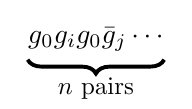
\begin{tikzpicture}[baseline={(trace.base)}]
    \node[inner sep=0pt] (trace) {%
      $g_0 g_i g_0 \bar{g}_j \cdots$};
    \draw [
      decorate,
      line width=1.4pt,
      decoration={
        brace,
        mirror,
        amplitude=5pt
      },
      transform canvas={yshift=-.2cm},
    ]
      (trace.south west) -- (trace.south east)
      node[midway,below=5pt,scale=0.9] {$n$ pairs};
  \end{tikzpicture} )
   = 2^{n-1} \tr(g_0 g_i) = 2^{n+1}.
\end{equation}

\subsection{A comment on gauge corrections} \label{sec:gauge_comment}

Before we finally state the N\textsuperscript{3}LO effective action for the cold
and dense regime we need to examine a final set of apparently low order graphs which
have yet to be discussed. They are the result of new geometries only possible to
construct with the insertion of plaquettes. The first of these appear at
$\mathcal{O}(\kappa^4 u)$ and is depicted to the far left in
\figref{fig:nontrivial-gauge}. This particular contribution arises in the
following integral
%
\begin{equation}
  \kappa^4 u\, \int_{\mathrlap{U}} \hskip .1cm \chi(U) \tr_{xsc} (P_i P_j M_i M_j), \hskip.5cm \text{ for } i \neq j.
\end{equation}
%
This however restricts the four quark hops to occupy the same temporal slice and
therefore only gives a single factor of $N_t$, while the dominating
$\mathcal{O}(\kappa^4)$ terms give contributions proportional to $N_t^2$. It is
possible to shift the quark hops on the slices by inserting plaquettes as can be
seen in the two other graphs in \figref{fig:nontrivial-gauge}, and would give a
correction to the formula above
%
\begin{equation}
  \kappa^4 u \bigg(1 + 2 \frac{u \kappa^2 - (u\kappa^2)^{N_t}}{1 - u\kappa^2} \bigg)^4 (1 + 4 u^5)
    \int_{\mathrlap{U}} \hskip .1cm \chi(U) \tr_{xsc} (P_i P_j M_i M_j),
\end{equation}
%
which of course would be highly suppressed as $u$ is also a small parameter.
This specific geometry will indeed appear at $\mathcal{O}(\kappa^8)$ where the
plaquette can be replaced by a quark loop including windings which can shift the
links arbitrarily in the temporal coordinate.

\begin{figure}
  {\centering
    \includegraphics[width=.95\textwidth]{non_trivial_gauge_corrections}\par}
  \caption{The three first non-trivial gauge corrections to
    $\mathcal{O}(\kappa^4)$}
  \label{fig:nontrivial-gauge}
\end{figure}

\subsection{The \texorpdfstring{$\mathcal{O}(\kappa^8)$}{O(k8)} effective action}

We finally turn our attention to the higher order contributions to the effective
theory. Although the groundwork has been laid, the combinatorics still have to
be carried out. As the number of terms grow exponentially, so does their
complexity, there is little chance for a straightforward computation ever to get
all the prefactors correct. Due to this, a computer program has been developed
as part of the present work. The aim is to compute the effective theory in the
limit of cold QCD \citep{jonas_rylund_glesaaen_2016_56319}.

The software computes the effective theory terms in a series of easily
understandable steps
%
\begin{enumerate}
  \item Computes all permutations of $P$ and $M$ that can enter a trace to a
    given order.
  \item Finds and collects all identical terms.
  \item Computes all combinations of traces of lower orders which give a
    contribution to the given order.
  \item Computes all contractions of $P$'s and $M$'s which can be realised
    spatially.
  \item Computes all spatial realisations of ambiguous multi trace contractions.
  \item Applies colour deltas from the spatial gauge integrals.
  \item Sums over all temporal permutations for every link.
\end{enumerate}
\begin{figure}
  {\centering
    \includegraphics[width=.6\textwidth]{spatial_contraction_examples}\par}
  \caption{The two possible spatial configurations of the contraction of
    $(\tr(P\,P\,M\,M))^2$ in \protect\meqref{eq:special-spatial-contraction}.}
  \label{fig:spatial-multitrace}
\end{figure}
%
The first three steps are essentially expanding the exponential as shown in
\meqref{eq:expanded_pm_notation}, while steps four and five loosely translate
to switching from the $PM$ notation to the contracted notation, as was
introduced in \secref{sec:combinatorics}. The fourth step can be amended by
placing a constriction on the contractions requiring an equal number of $P$ and
$M$ in between contractions, and requiring the spatial detour to return to its
starting point. For example
%
\begin{equation}
  \tikzset{
    every node/.style = {anchor=south, text depth=0.ex, inner sep=1pt}
  }
  \tr \begin{tikzpicture}[baseline={([yshift=1.5pt]one.south)}]
      \node (one) {$P$};
      \node (two) [right=0pt of one] {$P$};
      \node (three) [right=0pt of two] {$M$};
      \node (four) [right=0pt of three] {$M$};
      \path[contraction] (one.north) edge [skip loop=4pt] (three.north);
      \path[contraction] (two.north) edge [skip loop=8pt] (four.north);
    \end{tikzpicture}
\end{equation}
%
is an impossible contraction as the contracted $P$ and $M$ matrices can never
overlap. Contractions across multiple traces are more complicated as the traces
can be translated and rotated with respect to each other. An example of the
disambiguities can be seen in the $\mathcal{O}(\kappa^8)$ term
%
\begin{equation} \label{eq:special-spatial-contraction}
  \tikzset{
    every node/.style = {anchor=south, text depth=0.ex, inner sep=1pt}
  }
  \begin{tikzpicture}[baseline={([yshift=1.5pt]one.south)}]
      \node (tr1) {$\tr($};
      \node (one) [right=0pt of tr1,yshift=-1pt] {$P$};
      \node (two) [right=0pt of one] {$P$};
      \node (three) [right=0pt of two] {$M$};
      \node (four) [right=0pt of three] {$M$};
      \node (leftpar) [right=0pt of four,yshift=1pt] {$)$};
      \node (tr2) [right=.1cm of leftpar] {$\tr($};
      \node (five) [right=0pt of tr2,yshift=-1pt] {$P$};
      \node (six) [right=0pt of five] {$P$};
      \node (seven) [right=0pt of six] {$M$};
      \node (eight) [right=0pt of seven] {$M$};
      \node (leftpar2) [right=0pt of eight,yshift=1pt] {$)$};
      \path[contraction] (four.north) edge [skip loop=4pt] (five.north);
      \path[contraction] (three.north) edge [skip loop=8pt] (six.north);
      \path[contraction] (two.north) edge [skip loop=12pt] (seven.north);
      \path[contraction] (one.north) edge [skip loop=16pt] (eight.north);
    \end{tikzpicture},
\end{equation}
%
which has two possibilities for the spatial extent
%
\begin{equation}
  \tr(P_i P_j M_i M_j) \tr (P_j P_i M_j M_i) \hskip1ex\text{ and }\hskip1ex
  \tr(P_i P_j M_j M_i) \tr (P_i P_j M_j M_i).
\end{equation}
%
The graphical representation of the two choices are depicted in
\figref{fig:spatial-multitrace}. Summing over the colour indices from the gauge
link integral is simple, as we need only a single integral in the cold and dense
regime, namely the integral from \meqref{eq:uub-integral}
%
\begin{equation}
  I_{ij}^{kl} = \int \mathrm{d} U \, U_{ij} U^{\dagger}_{kl} = \frac{1}{N_c}
  \delta_{il} \delta_{jk}.
\end{equation}
%
After the computation has been carried out and equal terms have been collected,
we get the full effective action to a given order in $\kappa$ as output. The
number of terms at a given order is plotted in \figref{fig:number_of_terms}, in
which we see that it grows exponentially as we increase the expansion order.
This is a roadblock for the numerical evaluation as the number of operation one
has to do to compute the Monte Carlo weight / Complex Langevin force at some
point will overtake even that of computing the fermion determinant in full. The
number of terms can be reduced by around one order of magnitude by switching
between the two representations presented earlier and summing up equal terms,
but this is only a simplification for analytic evaluations as the numerical
work stays constant.

\begin{figure}
  {\centering
    \includegraphics[width=\textwidth]{hopping_number_of_terms}\par}
  \caption{Number of terms generated by the software at varying orders in
    $\kappa$.}
  \label{fig:number_of_terms}
\end{figure}

In \citep{Glesaaen:2015aaw,Glesaaen:2015vtp}, as well as in this thesis we work
with the effective action up to $\mathcal{O}(\kappa^8u^5)$.  Since the analytic
expression is rather lengthy, we give the effective action in a graphical
representation. This will also serve as a convenient notation for the analytic
evaluation, which we will tackle in the next session. The full expression will be
given in \apxref{apx:full_k8_action}. We symbolise factors of $W_{n,m}(\vec{x})$
by vertices where $n$ is the number of bonds entering a vertex and $m$ is the
number indicated on the node. Furthermore, vertices connected by one
or more nodes are nearest neighbours on the lattice
%
%\begingroup%
\allowdisplaybreaks%
\tikzset{
  circ/.style={%
    black,thick,circle,draw,inner sep=2pt,scale=0.75
  },
  midtikz/.style={
    baseline={([yshift=-.5ex]current bounding box.center)},
  },
}%
%\setlength{\medmuskip}{2mu}%
\medskip=2mu%
\begin{multline} \label{eq:effective_action_kapp8}
  S_{\mathrm{eff}} = S_0 + 
  h_2 N_f \sum_{\mathrm{dof}}  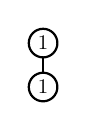
\begin{tikzpicture}[midtikz]
    \node[circ] (n1) {1};
    \node[circ] (n2) at ([shift={(270:.75)}] n1) {1}
      edge[thick] (n1);
  \end{tikzpicture}
   - h_2^2 N_f\sum_{\mathrm{dof}}  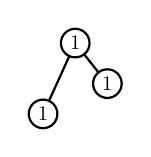
\begin{tikzpicture}[midtikz]
    \node[circ] (n1) {1};
    \node[circ] (n2) at ([shift={(60:{sqrt(2/3)})}] n1) {1}
      edge[thick] (n1);
    \node[circ] (n3) at ([shift={(300:{sqrt(2/3)})}] n2) {1}
      edge[thick] (n2);
  \end{tikzpicture}
  - h_2^2 N_f^2\sum_{\mathrm{dof}} 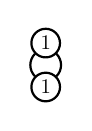
\begin{tikzpicture}[midtikz]
    \node[circ] (n1) {1};
    \node[circ] (n2) at ([shift={(270:.75)}] n1) {1}
      edge[thick,bend left=45] (n1)
      edge[thick,bend right=45] (n1);
  \end{tikzpicture}
  + h_2^3 N_f\sum_{\mathrm{dof}} 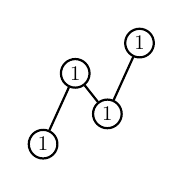
\begin{tikzpicture}[midtikz]
    \node[circ] (n1) {1};
    \node[circ] (n2) at ([shift={(60:{sqrt(2/3)})}] n1) {1}
      edge[thick] (n1);
    \node[circ] (n3) at ([shift={(300:{sqrt(2/3)})}] n2) {1}
      edge[thick] (n2);
    \node[circ] (n4) at ([shift={(60:{sqrt(2/3)})}] n3) {1}
      edge[thick] (n3);
  \end{tikzpicture} \\
  +\frac{1}{3} h_2^3 N_f \sum_{\mathrm{dof}} \Bigg( 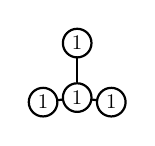
\begin{tikzpicture}[midtikz]
    \node[circ] (n1) {1};
    \node[circ] at ([shift={(-30:.5)}] n1) {1}
      edge[thick] (n1);
    \node[circ] at ([shift={(90:.5)}] n1) {1}
      edge[thick] (n1);
    \node[circ] at ([shift={(210:.5)}] n1) {1}
      edge[thick] (n1);
  \end{tikzpicture} 
  -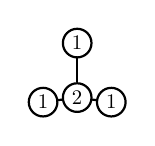
\begin{tikzpicture}[midtikz]
    \node[circ] (n1) {2};
    \node[circ] at ([shift={(-30:.5)}] n1) {1}
      edge[thick] (n1);
    \node[circ] at ([shift={(90:.5)}] n1) {1}
      edge[thick] (n1);
    \node[circ] at ([shift={(210:.5)}] n1) {1}
      edge[thick] (n1);
  \end{tikzpicture} \Bigg)
  +2 h_2^3 N_f^2 \sum_{\mathrm{dof}} \Bigg( 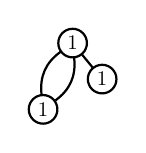
\begin{tikzpicture}[midtikz]
    \node[circ] (n1) {1};
    \node[circ] (n2) at ([shift={(60:.75)}] n1) {1}
      edge[thick,bend left=30] (n1)
      edge[thick,bend right=30] (n1);
    \node[circ] at ([shift={(300:.75)}] n2) {1}
      edge[thick] (n2);
  \end{tikzpicture} 
  - 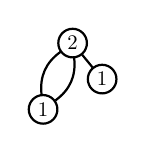
\begin{tikzpicture}[midtikz]
    \node[circ] (n1) {1};
    \node[circ] (n2) at ([shift={(60:.75)}] n1) {2}
      edge[thick,bend left=30] (n1)
      edge[thick,bend right=30] (n1);
    \node[circ] at ([shift={(300:.75)}] n2) {1}
      edge[thick] (n2);
  \end{tikzpicture} \Bigg) \\
  +\frac{1}{6} h_2^3 N_f \sum_{\mathrm{dof}} \Bigg( 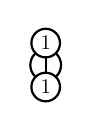
\begin{tikzpicture}[midtikz]
    \node[circ] (n1) {1};
    \node[circ] at ([shift={(270:.75)}] n1) {1}
      edge[thick,bend left=45] (n1)
      edge[thick,bend right=45] (n1)
      edge[thick] (n1);
  \end{tikzpicture} 
  - 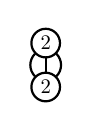
\begin{tikzpicture}[midtikz]
    \node[circ] (n1) {2};
    \node[circ] at ([shift={(270:.75)}] n1) {2}
      edge[thick,bend left=45] (n1)
      edge[thick,bend right=45] (n1)
      edge[thick] (n1);
  \end{tikzpicture} \Bigg)
  - \frac{4}{3} h_2^3 N_f^3 \sum_{\mathrm{dof}}  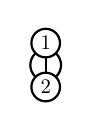
\begin{tikzpicture}[midtikz]
    \node[circ] (n1) {1};
    \node[circ] at ([shift={(270:.75)}] n1) {2}
      edge[thick,bend left=45] (n1)
      edge[thick,bend right=45] (n1)
      edge[thick] (n1);
  \end{tikzpicture} 
  - h_2^4 N_f\sum_{\mathrm{dof}} 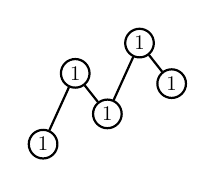
\begin{tikzpicture}[midtikz]
    \node[circ] (n1) {1};
    \node[circ] (n2) at ([shift={(60:{sqrt(2/3)})}] n1) {1}
      edge[thick] (n1);
    \node[circ] (n3) at ([shift={(300:{sqrt(2/3)})}] n2) {1}
      edge[thick] (n2);
    \node[circ] (n4) at ([shift={(60:{sqrt(2/3)})}] n3) {1}
      edge[thick] (n3);
    \node[circ] (n5) at ([shift={(300:{sqrt(2/3)})}] n4) {1}
      edge[thick] (n4);
  \end{tikzpicture} \\
  - \frac{1}{12} h_2^4 N_f\sum_{\mathrm{dof}} \Bigg( 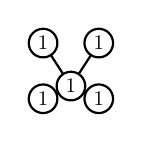
\begin{tikzpicture}[midtikz]
    \node[circ] (n1) {1};
    \node[circ] at ([shift={(45:.5)}] n1) {1}
      edge[thick] (n1);
    \node[circ] at ([shift={(135:.5)}] n1) {1}
      edge[thick] (n1);
    \node[circ] at ([shift={(225:.5)}] n1) {1}
      edge[thick] (n1);
    \node[circ] at ([shift={(315:.5)}] n1) {1}
      edge[thick] (n1);
  \end{tikzpicture}
  -2 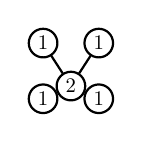
\begin{tikzpicture}[midtikz]
    \node[circ] (n1) {2};
    \node[circ] at ([shift={(45:.5)}] n1) {1}
      edge[thick] (n1);
    \node[circ] at ([shift={(135:.5)}] n1) {1}
      edge[thick] (n1);
    \node[circ] at ([shift={(225:.5)}] n1) {1}
      edge[thick] (n1);
    \node[circ] at ([shift={(315:.5)}] n1) {1}
      edge[thick] (n1);
  \end{tikzpicture}
  + 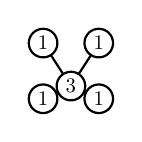
\begin{tikzpicture}[midtikz]
    \node[circ] (n1) {3};
    \node[circ] at ([shift={(45:.5)}] n1) {1}
      edge[thick] (n1);
    \node[circ] at ([shift={(135:.5)}] n1) {1}
      edge[thick] (n1);
    \node[circ] at ([shift={(225:.5)}] n1) {1}
      edge[thick] (n1);
    \node[circ] at ([shift={(315:.5)}] n1) {1}
      edge[thick] (n1);
  \end{tikzpicture} \Bigg)
  -  h_2^4 N_f\sum_{\mathrm{dof}} \Bigg( 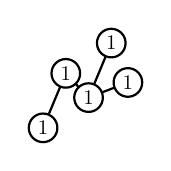
\begin{tikzpicture}[midtikz]
    \node[circ] (n1) {1};
    \node[circ] (n2) at ([shift={(60:{sqrt(1/3)})}] n1) {1}
      edge[thick] (n1);
    \node[circ] (n3) at ([shift={(300:{sqrt(1/3)})}] n2) {1}
      edge[thick] (n2);
    \node[circ] (n4) at ([shift={(60:{sqrt(1/3)})}] n3) {1}
      edge[thick] (n3);
    \node[circ] (n5) at ([shift={(0:.5)}] n3) {1}
      edge[thick] (n3);
  \end{tikzpicture}
  - 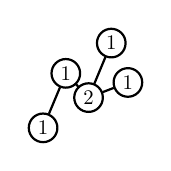
\begin{tikzpicture}[midtikz]
    \node[circ] (n1) {1};
    \node[circ] (n2) at ([shift={(60:{sqrt(1/3)})}] n1) {1}
      edge[thick] (n1);
    \node[circ] (n3) at ([shift={(300:{sqrt(1/3)})}] n2) {2}
      edge[thick] (n2);
    \node[circ] (n4) at ([shift={(60:{sqrt(1/3)})}] n3) {1}
      edge[thick] (n3);
    \node[circ] (n5) at ([shift={(0:.5)}] n3) {1}
      edge[thick] (n3);
  \end{tikzpicture} \Bigg) \\
  - h_2^4 N_f^2 \sum_{\mathrm{dof}} \Bigg( 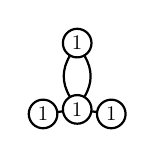
\begin{tikzpicture}[midtikz]
    \node[circ] (n1) {1};
    \node[circ] at ([shift={(-30:.5)}] n1) {1}
      edge[thick] (n1);
    \node[circ] at ([shift={(90:.65)}] n1) {1}
      edge[thick,bend left=30] (n1)
      edge[thick,bend right=30] (n1);
    \node[circ] at ([shift={(210:.5)}] n1) {1}
      edge[thick] (n1);
  \end{tikzpicture} 
  -4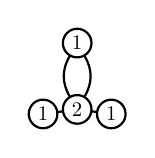
\begin{tikzpicture}[midtikz]
    \node[circ] (n1) {2};
    \node[circ] at ([shift={(-30:.5)}] n1) {1}
      edge[thick] (n1);
    \node[circ] at ([shift={(90:.65)}] n1) {1}
      edge[thick,bend left=30] (n1)
      edge[thick,bend right=30] (n1);
    \node[circ] at ([shift={(210:.5)}] n1) {1}
      edge[thick] (n1);
  \end{tikzpicture}
  +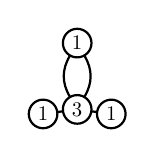
\begin{tikzpicture}[midtikz]
    \node[circ] (n1) {3};
    \node[circ] at ([shift={(-30:.5)}] n1) {1}
      edge[thick] (n1);
    \node[circ] at ([shift={(90:.65)}] n1) {1}
      edge[thick,bend left=30] (n1)
      edge[thick,bend right=30] (n1);
    \node[circ] at ([shift={(210:.5)}] n1) {1}
      edge[thick] (n1);
  \end{tikzpicture} \Bigg)
  - h_2^4 N_f^2 \sum_{\mathrm{dof}} 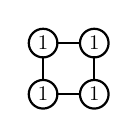
\begin{tikzpicture}[midtikz]
    \node[circ] (n1) {1};
    \node[circ] (n2) at (0.65,0) {1}
      edge[thick] (n1);
    \node[circ] (n3) at (0.65,0.65) {1}
      edge[thick] (n2);
    \node[circ] (n4) at (0,0.65) {1}
      edge[thick] (n3)
      edge[thick] (n1);
  \end{tikzpicture} \\
  -2 h_2^4 N_f^2 \sum_{\mathrm{dof}} \Bigg(  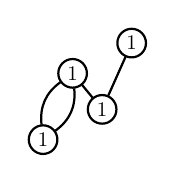
\begin{tikzpicture}[midtikz]
    \node[circ] (n1) {1};
    \node[circ] (n2) at ([shift={(60:.75)}] n1) {1}
      edge[thick,bend left=30] (n1)
      edge[thick,bend right=30] (n1);
    \node[circ] (n3) at ([shift={(300:.75)}] n2) {1}
      edge[thick] (n2);
    \node[circ] at ([shift={(60:.75)}] n3) {1}
      edge[thick] (n3);
  \end{tikzpicture}
  - 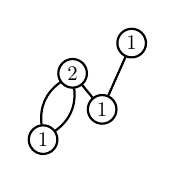
\begin{tikzpicture}[midtikz]
    \node[circ] (n1) {1};
    \node[circ] (n2) at ([shift={(60:.75)}] n1) {2}
      edge[thick,bend left=30] (n1)
      edge[thick,bend right=30] (n1);
    \node[circ] (n3) at ([shift={(300:.75)}] n2) {1}
      edge[thick] (n2);
    \node[circ] at ([shift={(60:.75)}] n3) {1}
      edge[thick] (n3);
  \end{tikzpicture} \Bigg)
  - h_2^4 N_f^2 \sum_{\mathrm{dof}} \Bigg(  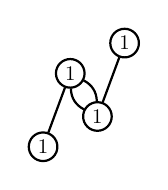
\begin{tikzpicture}[midtikz]
    \node[circ] (n1) {1};
    \node[circ] (n2) at ([shift={(65:{sqrt(2/3)})}] n1) {1}
      edge[thick] (n1);
    \node[circ] (n3) at ([shift={(-65:{sqrt(2/3)})}] n2) {1}
      edge[thick,bend left=30] (n2)
      edge[thick,bend right=30] (n2);
    \node[circ] (n4) at ([shift={(65:{sqrt(2/3)})}] n3) {1}
      edge[thick] (n3);
  \end{tikzpicture}
  -2 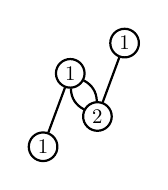
\begin{tikzpicture}[midtikz]
    \node[circ] (n1) {1};
    \node[circ] (n2) at ([shift={(65:{sqrt(2/3)})}] n1) {1}
      edge[thick] (n1);
    \node[circ] (n3) at ([shift={(-65:{sqrt(2/3)})}] n2) {2}
      edge[thick,bend left=30] (n2)
      edge[thick,bend right=30] (n2);
    \node[circ] (n4) at ([shift={(65:{sqrt(2/3)})}] n3) {1}
      edge[thick] (n3);
  \end{tikzpicture}
  + \begin{tikzpicture}[midtikz]
    \node[circ] (n1) {1};
    \node[circ] (n2) at ([shift={(65:{sqrt(2/3)})}] n1) {2}
      edge[thick] (n1);
    \node[circ] (n3) at ([shift={(-65:{sqrt(2/3)})}] n2) {2}
      edge[thick,bend left=30] (n2)
      edge[thick,bend right=30] (n2);
    \node[circ] (n4) at ([shift={(65:{sqrt(2/3)})}] n3) {1}
      edge[thick] (n3);
  \end{tikzpicture} \Bigg) \\
  -\frac{1}{3} h_2^4 N_f \sum_{\mathrm{dof}} \Bigg(  \begin{tikzpicture}[midtikz]
    \node[circ] (n1) {1};
    \node[circ] (n2) at ([shift={(60:.75)}] n1) {1}
      edge[thick,bend left=30] (n1)
      edge[thick,bend right=30] (n1)
      edge[thick] (n1);
    \node[circ] (n3) at ([shift={(300:.75)}] n2) {1}
      edge[thick] (n2);
  \end{tikzpicture}
  -2 \begin{tikzpicture}[midtikz]
    \node[circ] (n1) {1};
    \node[circ] (n2) at ([shift={(60:.75)}] n1) {2}
      edge[thick,bend left=30] (n1)
      edge[thick,bend right=30] (n1)
      edge[thick] (n1);
    \node[circ] (n3) at ([shift={(300:.75)}] n2) {1}
      edge[thick] (n2);
  \end{tikzpicture}
  +2 \begin{tikzpicture}[midtikz]
    \node[circ] (n1) {2};
    \node[circ] (n2) at ([shift={(60:.75)}] n1) {2}
      edge[thick,bend left=30] (n1)
      edge[thick,bend right=30] (n1)
      edge[thick] (n1);
    \node[circ] (n3) at ([shift={(300:.75)}] n2) {1}
      edge[thick] (n2);
  \end{tikzpicture}
  - \begin{tikzpicture}[midtikz]
    \node[circ] (n1) {2};
    \node[circ] (n2) at ([shift={(60:.75)}] n1) {3}
      edge[thick,bend left=30] (n1)
      edge[thick,bend right=30] (n1)
      edge[thick] (n1);
    \node[circ] (n3) at ([shift={(300:.75)}] n2) {1}
      edge[thick] (n2);
  \end{tikzpicture} \Bigg) \\
  +\frac{4}{3} h_2^4 N_f^3 \sum_{\mathrm{dof}} \Bigg(  \begin{tikzpicture}[midtikz]
    \node[circ] (n1) {2};
    \node[circ] (n2) at ([shift={(60:.75)}] n1) {1}
      edge[thick,bend left=30] (n1)
      edge[thick,bend right=30] (n1)
      edge[thick] (n1);
    \node[circ] (n3) at ([shift={(300:.75)}] n2) {1}
      edge[thick] (n2);
  \end{tikzpicture}
  -2 \begin{tikzpicture}[midtikz]
    \node[circ] (n1) {2};
    \node[circ] (n2) at ([shift={(60:.75)}] n1) {2}
      edge[thick,bend left=30] (n1)
      edge[thick,bend right=30] (n1)
      edge[thick] (n1);
    \node[circ] (n3) at ([shift={(300:.75)}] n2) {1}
      edge[thick] (n2);
  \end{tikzpicture}
  +2 \begin{tikzpicture}[midtikz]
    \node[circ] (n1) {1};
    \node[circ] (n2) at ([shift={(60:.75)}] n1) {2}
      edge[thick,bend left=30] (n1)
      edge[thick,bend right=30] (n1)
      edge[thick] (n1);
    \node[circ] (n3) at ([shift={(300:.75)}] n2) {1}
      edge[thick] (n2);
  \end{tikzpicture}
  - \begin{tikzpicture}[midtikz]
    \node[circ] (n1) {1};
    \node[circ] (n2) at ([shift={(60:.75)}] n1) {3}
      edge[thick,bend left=30] (n1)
      edge[thick,bend right=30] (n1)
      edge[thick] (n1);
    \node[circ] (n3) at ([shift={(300:.75)}] n2) {1}
      edge[thick] (n2);
  \end{tikzpicture} \Bigg) \\
  -\bigg(\frac{1}{12} N_f + \frac{2}{3} N_f^3 \bigg) h_2^4 \sum_{\mathrm{dof}} \Bigg(  \begin{tikzpicture}[midtikz]
    \node[circ] (n1) {1};
    \node[circ] (n2) at ([shift={(60:.75)}] n1) {1}
      edge[thick,bend left=30] (n1)
      edge[thick,bend right=30] (n1);
    \node[circ] (n3) at ([shift={(300:.75)}] n2) {1}
      edge[thick,bend left=30] (n2)
      edge[thick,bend right=30] (n2);
  \end{tikzpicture}
  -4 \begin{tikzpicture}[midtikz]
    \node[circ] (n1) {1};
    \node[circ] (n2) at ([shift={(60:.75)}] n1) {2}
      edge[thick,bend left=30] (n1)
      edge[thick,bend right=30] (n1);
    \node[circ] (n3) at ([shift={(300:.75)}] n2) {1}
      edge[thick,bend left=30] (n2)
      edge[thick,bend right=30] (n2);
  \end{tikzpicture}
  + \begin{tikzpicture}[midtikz]
    \node[circ] (n1) {1};
    \node[circ] (n2) at ([shift={(60:.75)}] n1) {3}
      edge[thick,bend left=30] (n1)
      edge[thick,bend right=30] (n1);
    \node[circ] (n3) at ([shift={(300:.75)}] n2) {1}
      edge[thick,bend left=30] (n2)
      edge[thick,bend right=30] (n2);
  \end{tikzpicture} \Bigg)  \\
  -\frac{2}{3} h_2^4 N_f^4 \sum_{\mathrm{dof}} \Bigg(  \begin{tikzpicture}[midtikz]
    \node[circ] (n1) {1};
    \node[circ] (n2) at (0,-.75) {3}
      edge[thick, bend right=45] (n1)
      edge[thick, bend left=45] (n1)
      edge[thick, bend right=15] (n1)
      edge[thick, bend left=15] (n1);
  \end{tikzpicture}
  +2 \begin{tikzpicture}[midtikz]
    \node[circ] (n1) {2};
    \node[circ] (n2) at (0,-.75) {2}
      edge[thick, bend right=45] (n1)
      edge[thick, bend left=45] (n1)
      edge[thick, bend right=15] (n1)
      edge[thick, bend left=15] (n1);
  \end{tikzpicture} \Bigg)
  -\frac{1}{12} h_2^4 N_f^2 \sum_{\mathrm{dof}} \Bigg(  \begin{tikzpicture}[midtikz]
    \node[circ] (n1) {1};
    \node[circ] (n2) at (0,-.75) {1}
      edge[thick, bend right=45] (n1)
      edge[thick, bend left=45] (n1)
      edge[thick, bend right=15] (n1)
      edge[thick, bend left=15] (n1);
  \end{tikzpicture}
  +12 \begin{tikzpicture}[midtikz]
    \node[circ] (n1) {2};
    \node[circ] (n2) at (0,-.75) {2}
      edge[thick, bend right=45] (n1)
      edge[thick, bend left=45] (n1)
      edge[thick, bend right=15] (n1)
      edge[thick, bend left=15] (n1);
  \end{tikzpicture}
  + \begin{tikzpicture}[midtikz]
    \node[circ] (n1) {3};
    \node[circ] (n2) at (0,-.75) {3}
      edge[thick, bend right=45] (n1)
      edge[thick, bend left=45] (n1)
      edge[thick, bend right=15] (n1)
      edge[thick, bend left=15] (n1);
  \end{tikzpicture} \Bigg)  \\
  +\frac{2}{3} h_2^4 N_f^2 \sum_{\mathrm{dof}} \Bigg(  \begin{tikzpicture}[midtikz]
    \node[circ] (n1) {1};
    \node[circ] (n2) at (0,-.75) {2}
      edge[thick, bend right=45] (n1)
      edge[thick, bend left=45] (n1)
      edge[thick, bend right=15] (n1)
      edge[thick, bend left=15] (n1);
  \end{tikzpicture}
  + \begin{tikzpicture}[midtikz]
    \node[circ] (n1) {2};
    \node[circ] (n2) at (0,-.75) {3}
      edge[thick, bend right=45] (n1)
      edge[thick, bend left=45] (n1)
      edge[thick, bend right=15] (n1)
      edge[thick, bend left=15] (n1);
  \end{tikzpicture} \Bigg) +\mathcal{O} \big(\kappa^{10}, \frac{1}{N_{\tau}}\big).
\end{multline}
\endgroup%

\begin{equation} \label{eq:effective_action_kapp8}
  \tikz \node[anchor=base, baseline, minimum width=.9\textwidth, draw, minimum height=2cm, ColourHl1,thick] {Dummy equation}; 
\end{equation}
%
The sums over "degrees of freedom" represent the remaining spatial trace, which
remains to be carried out either for analytic computations or during numerical
evaluation. We see that all the higher order interactions appear with a coupling
constant equal to some power of the nearest neighbour coupling constant $h_2$. This
is not very hard to see mathematically, as every new spatial link contributes a
combinatorial factor of $N_t$, a hopping factor of $\kappa^2$ and the gauge
integration results in a factor of $N_c^{-1}$ for every integrated link.
Since no spatial links ever overlap, we can apply gauge corrections on a
link by link basis regardless of whether they connect the same nearest neighbour
sites. Corrections to this will appear at NLO in $N_t^{-1}$. The gauge
corrections are therefore given by replacing $h_2 \to h_2(\beta)$ as given by
\meqref{eq:h2_gauge_corrections}.

\subsection{Application region of the large-$N_t$ approximation}

Although there is no questioning the dense approximation for its region of
applicability when studying the cold and dense regim due to its exponential nature,
one might ask the validity of the expansion around $N_t^{-1} \to 0$. The lowest
order correction to this limit comes at order $\kappa^4 N_t$. If we choose a
somewhat extreme scenario for our parameters, $h_2 = 0.15$ and $N_t = 50$, we
see that the $\kappa^4 N_t$ and $h_2^4$ have about the same order of magnitude,
meaning that the next order in $N_t^{-1}$ should contribute about the same as
the $\kappa^8$ terms do. To analyse this effect we plot the ratio of the baryon
number density computed at fixed $h_1$ and $h_2$ using the $\mathcal{O}(h_2^4)$
action with and without the $\mathcal{O}(\kappa^4 N_t)$ terms, shown in
\figref{fig:nb_of_nt_comparison}. Although the prefactor of the expansion
coefficients are around the same order of magnitude, it is clear that the
contributions from these higher order terms give small corrections to the final
result. Already at $N_t \leq 13$ the contribution is less than $5 \%$, which is
insignificant when compared to the contribution from the $\mathcal{O}(h_2^4)$
term at these extreme parameter choices. We thus conclude that the large-$N_t$
limit is well under control for the physical region we are studying.

\begin{figure}[t]
  \begin{center}
    \begin{adjustbox}{max width=\textwidth}
      \includegraphics[width=0.6\textwidth]{nb_of_nt_comparison}
    \end{adjustbox}
  \end{center} \vskip -.5cm
  \caption{Ratio of baryon number density at $\mathcal{O}(h_2^4, \kappa^4 N_t)$
    and at $\mathcal{O}(h_2^4)$ for fixed $h_1$ and $h_2$ in the strong coupling
    limit. Computed with the analytic treatment of \protect\chapref{chap5}.}
  \label{fig:nb_of_nt_comparison}
\end{figure}


\section{Numerical evaluation} \label{sec:numerical_evaluation}

Although the focus of this thesis is the analytic evaluation of the effective
theory, a couple of remarks on the numerical evaluation is still in order.  At
the beginning of this chapter we stated the nefarious sign problem as a
motivation for developing the effective 3D theory. And although the effective
theory still suffers from a conceptual sign problem in the sense that the action
take complex values, we are in a regime where methods such as reweighting work
well.  A thorough review of the theory's numerical properties can be found in
\citep{Neuman:2015zb}.

The effective theory offers multiple advantages for numerical evaluation over
full lattice calculations besides the apparent resolution of the sign problem.
%
\begin{itemize}
  \item First and foremost we have replaced the very expensive fermion
    determinant with a discrete sum over the volume and a handful of terms, an
    overall much cheaper computation.
  \item Second, the temporal direction has been integrated out and its remnant is
    encoded in $N_t$, which is a parameter, reducing the dimensionality of the
    variable space by one.
  \item Finally, the remaining field variables are traces of group elements of
    SU($3$) which can be represented by two real angles in comparison to the
    eight generators needed to represent a gauge link in full lattice QCD.
\end{itemize}
%
Regardless of whether one chooses to do a reweighted \emph{Monte Carlo} (MC) or
a \emph{Complex Langevin} (CL) simulation to deal with the trivial sign problem,
it is advantageous to rewrite the partition function to depend on the angular
representation of the group characters, as outlined in \apxref{sec:haar_measure}.
For SU($3$) we replace the characters with
%
\begin{equation}
  L(\vec{x}) \equiv \chi_1 = e^{i \theta_{\vec{x}}} + e^{i \phi_{\vec{x}}} +
  e^{-i(\theta_{\vec{x}} + \phi_{\vec{x}})}
\end{equation}
%
and the integration measure by
%
\begin{equation}
  \int [\mathrm{d} W]_{\vec{x}} = \frac{1}{(2\pi)^2 N_c!}\int \prod_{\vec{x}} \mathrm{d} \theta_{\vec{x}}
  \mathrm{d} \phi_{\vec{x}} H(\theta_{\vec{x}}, \phi_{\vec{x}})
\end{equation}
%
where $H$ is the reduced Haar measure given by \meqref{eq:su3-haar-measure}.
This induces a Polyakov Loop potential in the action
%
\begin{equation}
  \int \big[ \mathrm{d} \theta\, \mathrm{d} \phi \big]_{\vec{x}} \,
    e^{-S_{\text{eff}} + V[L]},
\end{equation}
%
with the potential as stated in the appendix
%
\begin{equation}
  V[L] = \log ( \sum_{\vec{x}} 27 - 18 |L(\vec{x})|^2 + 8 \mathrm{Re} \, L(\vec{x})^3 - |L(\vec{x})|^4 )\,.
\end{equation}
%
The effective theory is also easily extendable to other gauge groups,
especially other SU($N_c$). One simply has to give the proper reduced Haar
measure and give the definition for the new Polyakov loop variable
%
\begin{equation}
  L_{N_c}(\vec{x}) = \sum_{n=1}^{N_c-1} e^{i \theta_n(\vec{x})} + e^{-i
    \sum_{n=1}^{N_c-1} \theta_n (\vec{x})}.
\end{equation}
%
We see that an effective theory using the gauge group SU($N_c$) has
$N_s^3(N_c-1)$ degrees of freedom as compared to the $4 N_s^3 N_t (N_c^2 - 1)$
degrees of freedom one would have in a full lattice gauge theory simulation.
Therefore, on top of the reduced computation cost the theory also scales
linearly in complexity with the number of colours as compared to quadratic in a
full simulation.

\begin{figure}
  \begin{center}
    \begin{adjustbox}{max width=.99\textwidth}
      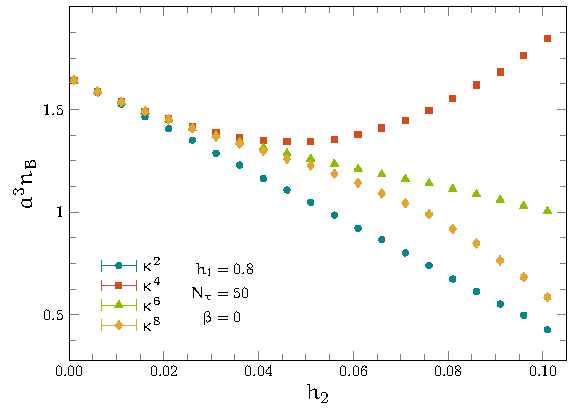
\includegraphics{convergence_numeric_kappa}
      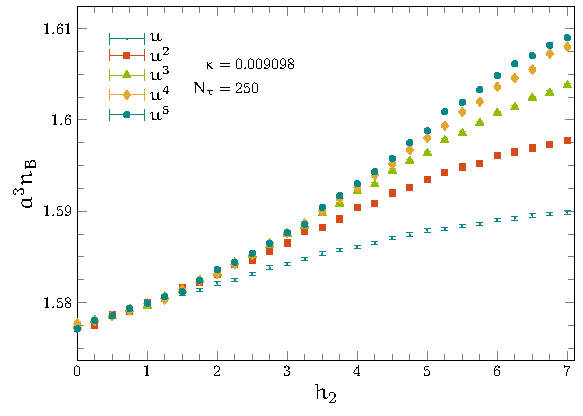
\includegraphics{convergence_numeric_beta}
    \end{adjustbox}
  \end{center}\vskip -.5cm
  \caption[
    Left: Convergence of baryon number density in lattice units as a
      function of the nearest neighbour coupling $h_2$ in various orders of the
      hopping expansion at strong coupling. Right: Corresponding convergence plot
      at different orders in the character expansion parameter $u$.
  ]{
    Left: Convergence of baryon number density in lattice units as a
    function of the nearest neighbour coupling $h_2$ in various orders of the
    hopping expansion at strong coupling. Right: Corresponding convergence plot
    at different orders in the character expansion parameter $u$
    \protect\footnotemark.}
  \label{fig:numerical_convergence}
\end{figure}
%
The simulations were carried out using both algorithms, MC with reweighting and
CL, and the results were cross checked \citep{Langelage:2014vpa}. Both methods
give compatible results within the parameter range for which the effective
theory is well defined. Our first task is to assess the range of validity of the
strong coupling, heavy quark action. One expects the additional orders in
$\kappa$ to extend the convergence region, within which the description of
thermodynamic functions by the effective action is reliable. We test this by
computing the baryon number density at fixed values of the coupling $h_1$ and
$N_{\tau}$.  Varying $\kappa$ then allows us to assess the convergence of the
expansion of the kinetic quark determinant.  \figref{fig:numerical_convergence}
(left) shows the results obtained with effective actions of increasing order in
$\kappa$. One clearly observes how two adjacent orders stay together for larger
values of $h_2(\kappa)$ as the order increase, thus extending the range where
our effective action is reliable.  \figref{fig:numerical_convergence} (right)
shows the same exercise for the largest $\kappa$ considered in this work, this
time increasing the orders of the character expansion. We observe good
convergence up to $\beta\sim 6$, which is a sufficiently weak coupling to allow
for continuum extrapolations. It is interesting to note that the convergence
properties are not determined by the size of the expansion parameters alone.
Even though the $u(\beta)$-values far exceed the $\kappa$-values employed in the
figures, convergence in $u(\beta)$ appears to be faster.  The gain in
convergence region by the additional orders in the effective action can be
exploited to study the systematics of our effective theory.
%
\footnotetext{Siumulation data courtesy of Mathias Neuman}

We will leave the numeric evaluation for now and will shift our focus to a
purely analytical treatment of the effective 3D theory using graphical methods
borrowed from the linked cluster formalism.
